% %%
\documentclass[lettersize,journal]{IEEEtran}
%\documentclass[lettersize,journal,draft]{IEEEtran}

\usepackage{amsmath,amsfonts,amssymb}
\usepackage{algorithmic}
\usepackage{array}
\usepackage{textcomp}
\usepackage{stfloats}
\usepackage{url}
\usepackage{verbatim}
\usepackage{graphicx}
\usepackage{cite}
\usepackage{balance}
\newtheorem{theorem}{Theorem}
\newtheorem{proposition}{Proposition}
\newtheorem{lemma}{Lemma}
\newtheorem{corollary}{Corollary}
\newtheorem{remark}{Remark}
\newtheorem{assumption}{Assumption}
\hyphenation{op-tical net-works semi-conduc-tor IEEE-Xplore}
\def\BibTeX{{\rm B\kern-.05em{\sc i\kern-.025em b}\kern-.08em
    T\kern-.1667em\lower.7ex\hbox{E}\kern-.125emX}}

\urlstyle{same}
\begin{document}

\title{Adaptive Navigation along the Separatrix of the Double Gyre}

\author{Christopher Waight and Christopher A. Kitts,~\IEEEmembership{Senior Member,~IEEE}
\thanks{Manuscript received Month Day, Year; revised Month Day, Year.}
\thanks{C. Waight is a PhD Candidate in the Robotic Systems Laboratory, Department of Mechanical
Engineering, Santa Clara University, Santa Clara, CA 95053 USA (e-mail: cwaight@scu.edu)}
\thanks{C. A. Kitts is Professor and Director of the Robotic Systems Laboratory, Department of
Mechanical Engineering, Santa Clara University, Santa Clara, CA 95053 USA (e-mail: ckitts@scu.edu)}
}
\markboth{Journal of \LaTeX\ Class Files,~Vol.~XX, No.~X, Month~Year}%
{Waight and Kitts: Adaptive Navigation along the Separatrix of the Double Gyre}

\maketitle

% ---------------------------------------------------------------------------
\begin{abstract}
Objective Eulerian coherent structures (OECSs) are short-term,
frame-invariant transport barriers that organize instantaneous material
transport in general dynamical systems. They can be viewed as the
instantaneous counterparts of stable and unstable manifolds, extracted
from the rate-of-strain field at a single instant rather than from
trajectories integrated over a finite horizon. Identifying OECSs is
useful for applications that demand short-term or real-time forecasting,
including oceanography and weather prediction. In this paper, we present
a collaborative robotic control strategy that tracks the short-term
attracting and repelling structures of a flow, including ocean flows,
without prepositioning the robots and without requiring global
information about the dynamics; it relies instead on local sensing,
prediction, and correction. For the two-dimensional incompressible flows
we consider, the determinant of the flow Jacobian, equivalently the
Okubo-Weiss field, is a signed scalar surrogate whose valley lines
(trenches) mark the strongest hyperbolicity, where the hyperbolic OECS
resides. We develop an adaptive controller built on a modified Newton
step: rather than steepest descent or ascent, the step reweights the
search directions so the team snaps onto the trench more rapidly and
slides along the structure, through a saddle point of this scalar
field, and down the opposing branch. The strategy is implemented with a
team of six robots and validated on a time-dependent model of a
wind-driven double-gyre flow and on actual ocean-flow data. We present
simulation results and discuss theoretical guarantees of the
collaborative tracking strategy.
\end{abstract}

\begin{IEEEkeywords}
Multirobot Systems, Adaptive Navigation, Vector Fields, Separatrix,
Double Gyre, Critical Points, Cooperative Estimation, Cluster Control
\end{IEEEkeywords}


% ---------------------------------------------------------------------------
\section{Introduction}
\label{sec:intro}

\IEEEPARstart{M}{ultirobot} systems exploit spatial distribution across a team to sample
and act on an environment more effectively than a single platform can, a
capability with broad application to formation assembly, coverage, and
distributed sensing \cite{1}. Deployed in geophysical flows such as ocean
currents and atmospheric jets, these teams often need to locate and track
dynamically meaningful boundaries rather than isolated critical points.
Coordinated multi-vehicle sampling of dynamic ocean features is itself an
active area of marine robotics, from drifter-referenced AUV surveys of
advecting patches \cite{2} to heterogeneous ASV/AUV teams tracking salinity
fronts \cite{3} and glider fleets adaptively sampling upwelling events during
the AOSN-II experiment in Monterey Bay \cite{4}. A boundary that appears
prominently in steady two-dimensional flows is the separatrix, which
contains both the stable and unstable manifold connecting to saddle
points and partitions the domain into two distinct basins. Tracking it
is relevant to dispersion modeling, pollutant containment, and the
deployment of sensor networks in coastal and atmospheric environments
\cite{6,7,8}, and, like the related Okubo-Weiss field used to detect and
classify oceanic mesoscale eddies \cite{5}, it can in principle be inferred
from instantaneous field measurements alone.

A line of work has equipped robot teams to track a coherent structure directly
in the flow rather than reconstruct it offline. Michini et al. straddle a
presumed stable or unstable manifold with a three-robot, PIM-triple-inspired
formation, using only local velocity measurements to keep one robot near the
manifold and the other two on opposite sides of it \cite{9}; the same strategy was
extended to an $N$-robot team for finer spatial sampling of the same manifold
\cite{10} and validated on physical micro-ASVs in a flow tank \cite{11}. Knizhnik et al.
couple a related manifold-tracking law to vehicle-level flow control in
gyre-like marine environments \cite{12}. Kularatne and Hsieh take a different
approach, computing the local finite-time Lyapunov exponent field on board
from the team's own accumulated velocity measurements, which recovers the
structure's type explicitly rather than assuming it \cite{13}. Every member of this
family, however, fixes the structure's identity before tracking begins: \cite{9},
\cite{10}, and \cite{11} require a saddle-straddling line segment seeded around an
already-assumed manifold, and their controller commits in advance to
tracking either the stable or the unstable branch, since the team's estimate
of the manifold's location is read off as the point of maximum measured speed
along the straddle segment if the unstable manifold is being tracked, or of
minimum speed if the stable manifold is being tracked. Neither the controller
nor its stability proof addresses what happens when the tracked branch
reaches a saddle, where this choice becomes ambiguous, since the straddle
segment's validity proof assumes it crosses the manifold exactly once and
stops there. Kularatne and Hsieh's onboard FTLE estimate avoids fixing the
structure's type in advance, but only by accumulating a velocity time history
over a finite integration horizon before an estimate is well formed, an
approach discussed further in Section~\ref{sec:separatrix}. This paper's
estimator and controller require neither a seeded manifold nor an
integration horizon: from an arbitrary six-robot configuration, they infer a
structure's location, its type, and, at a crossing, which branch to continue
onto, from the current instantaneous measurement alone.

Our own prior work estimated a single isolated critical point and classified
it from the eigenvalues of a linear Jacobian fit, using a three-robot
formation and a proportional or orbital control law \cite{14}. That is a
point-estimation problem. The work presented here is a field-structure
problem: it fits a quadratic model of the vector field, derives the
curvature of $\det(\mathbf{J})$ from that fit, and uses the curvature to
track a one-dimensional manifold rather than converge to a point.

This paper presents the following contributions:
\begin{enumerate}
    \item A distributed quadratic estimator that uses simultaneous measurements
          from six omnidirectional robots to recover the Jacobian $\mathbf{J}$,
          the determinant $\det(\mathbf{J})$, its gradient
          $\nabla\det(\mathbf{J})$, and its Hessian $\mathbf{H}_D$ at the cluster
          centroid, with no prior knowledge of the field. We prove six robots
          are the exact minimum for the coupled two-component case, one more
          than the five-plus-center formation sufficient for a single scalar
          field \cite{15}, and derive $\det(\mathbf{J})$, its gradient, and its
          Hessian analytically by differentiating through the jointly fitted
          vector coefficients, rather than by fitting a scalar surrogate
          directly.
    \item A hybrid three-mode separatrix tracker (Logic C) built on a
          modified Newton step: the ordinary step
          $-\mathbf{H}_D^{-1}\nabla D$ is decomposed in the eigenbasis of
          $\mathbf{H}_D$, each eigen-direction is independently saturated,
          and each signed eigenvalue is replaced by its magnitude so the
          team slides along a trench even where the local curvature is
          negative. The result is a controller that snaps onto the trench,
          slides along the stable manifold of the double-gyre saddle, and
          carries a flow-assisted mode across the crest where the
          along-trench gradient vanishes.
    \item A stability and network-traversal proof for the separatrix tracker:
          the trench a controller reaches continues through every saddle it
          crosses, with single-saddle capture recovered only as a
          tightened-threshold special case. Unlike prior manifold trackers,
          which fix the tracked branch's identity before the run begins
          \cite{9,10}, this controller commits to no manifold identity in
          advance, so the branch to continue onto at a crossing is read from
          the same instantaneous fit that located the crossing, rather than
          assumed ahead of time.
    \item Monte Carlo simulation validation of the controller under a fully
          specified noise model, with a success-rate map over a two-dimensional
          sweep of measurement and position noise standard deviations, and
          demonstration of effectiveness on real oceanic current data.
          Hardware validation is discussed as future work
          (Section~\ref{sec:future}).
\end{enumerate}

The remainder of the paper is organized as follows. The rest of this
section reviews related work. Section~\ref{sec:detj_field} formulates the
problem, describing the double-gyre model, the $\det(\mathbf{J})$ field, and
the separatrix as an Eulerian trench.
Section~\ref{sec:estimation} develops the six-robot quadratic estimator
and its sensitivity. Section~\ref{sec:controllers} presents the adaptive
separatrix controller.
Section~\ref{sec:stability} provides stability proofs.
Section~\ref{sec:methods} describes the simulation program, noise model, and
testing plan. Section~\ref{sec:results} presents results.
Section~\ref{sec:discussion} discusses implications and failure modes.
Sections~\ref{sec:limitations} and \ref{sec:future} cover limitations and
future work. Section~\ref{sec:conclusion} concludes.


% ---------------------------------------------------------------------------

\subsection{Lagrangian Coherent Structures and the Objectivity Question}

Haller and Yuan formalized the modern notion of a Lagrangian coherent
structure (LCS) as the extension of a stable or unstable manifold to flows
with arbitrary time dependence, a distinguished material surface that
organizes tracer transport over a finite time horizon \cite{6}. Haller's later
review frames the resulting body of theory as the search for the Lagrangian
skeleton of a flow, and states the property such a skeleton must have to be
physically meaningful: objectivity, invariance under the time-dependent
Euclidean frame changes that a material response cannot depend on \cite{16}.
Shadden, Lekien, and Marsden gave the standard computable definition, an LCS
as a ridge of the finite-time Lyapunov exponent (FTLE) field, and verified it
on the same double-gyre model used throughout this paper, where for
$\varepsilon > 0$ the ridge tracks the underlying heteroclinic connection
\cite{8}. Both the definition and its objectivity come at a fixed cost: an FTLE
ridge is a property of particle trajectories integrated over a finite
horizon, so extracting one requires the velocity field's future evolution
over that horizon, in advance, everywhere the tracers travel. Haller's
review is explicit that this is why the classical instantaneous criteria,
including Okubo-Weiss, the Q-criterion, and the Hua-Klein criterion, are
excluded from the Lagrangian framework entirely: they can frame a coherent
feature of the instantaneous velocity field, but they are not objective
\cite{16}. Serra and Haller later placed a version of this instantaneous idea on
objective footing with objective Eulerian coherent structures (OECSs),
constructed from the spin and rate-of-strain tensors rather than the raw
velocity gradient, and showed OECSs are the limit LCSs approach as the
integration horizon shrinks to zero, a limit Nolan, Serra, and Ross later
made precise for the FTLE field itself \cite{17,18}. The velocity gradient
that this instantaneous cost is paid to avoid is itself hard to obtain from
trajectory data alone: Harms, Dawson, and McKeon show that standard
gradient-based LCS diagnostics degrade badly on the sparse tracer
trajectories typical of ocean drifters, and propose a regression-based
alternative that linearizes in time rather than in space to recover usable
gradients from sparse data \cite{19}. The rate-of-strain and spin decomposition
underlying all of these instantaneous diagnostics is itself the subject of
ongoing refinement; Haller's dynamic polar decomposition, for instance,
identifies a mean material rotation rate that agrees with the classical
vorticity-based rate used throughout this paper while correcting a
memory effect present in the standard polar decomposition of the
deformation gradient \cite{20}. A robot team sampling the flow once per
control cycle, with no forecast, sits on the instantaneous side of the
resulting tradeoff, objectivity and material accuracy against zero
integration latency, by construction; this paper adopts that side
deliberately and returns to what is gained and given up by the choice in
Section~\ref{sec:separatrix}.

\subsection{Eulerian Surrogates: Okubo-Weiss, Q-Criterion, Hua-Klein}

Okubo and, independently, Weiss proposed the pointwise criterion
$Q = \tfrac{1}{4}(s_n^2 + s_s^2 - \omega^2)$ to partition a two-dimensional
flow into rotation-dominated and strain-dominated regions using only the
local velocity gradient, with their sign convention marking vortex cores by
$Q < 0$ \cite{21,22}. Hunt, Wray, and Moin generalized the same second-invariant
idea to three dimensions as the Q-criterion for identifying eddies, streams,
and convergence zones in turbulent flow fields \cite{23}. Hua and Klein revisited
the two-dimensional criterion for oceanographic use, sharpening the
conditions under which it correctly separates elliptic and hyperbolic
regions of a nearly two-dimensional turbulent flow \cite{24}. This paper works
with $D = \det(\mathbf{J})$ rather than $Q$; for the incompressible flows
considered here the two carry identical information with opposite sign,
$Q = -D$ (Section~\ref{sec:detj_field}), so $D > 0$ marks vortex cores and
$D < 0$ marks strain-dominated regions throughout. What every criterion in
this family shares, and what distinguishes it from the FTLE ridges of
Section~\ref{sec:separatrix}, is that each is a scalar function of the
pointwise velocity-gradient tensor, requiring only the instantaneous field
at a point, not an integration over time. Approaches that reduce a sensed
vector field to a scalar this way lose more than time dependence, however:
Cooper et al.'s initial multirobot study of vector field navigation reduced
each measurement to its magnitude, which yields a descent direction but
cannot distinguish a sink from a saddle from a vortex, since the magnitude
vanishes at every critical point regardless of type \cite{25}. Rather than
sensing a scalar reduction of the field directly, whether a speed magnitude
or an Okubo-Weiss-type invariant, we estimate the full local quadratic
vector field and obtain $D$, $\nabla D$, and $\mathbf{H}_D$ as derived
quantities from the jointly fitted components of $u$ and $v$
(Section~\ref{sec:estimation}), which is what makes the surrogate's
gradient and curvature, not merely its sign, available to the controller.

\subsection{Robots Tracking Manifolds and Coherent Structures}

The nearest prior work to this paper tracks a coherent structure directly
with a robot formation rather than computing it offline. Michini, Hsieh,
Forgoston, and Schwartz proposed a PIM-triple-inspired saddle straddle:
three robots bracket a presumed stable or unstable manifold, using only
local velocity measurements to keep one robot on the manifold and the other
two on either side of it, with no FTLE field or global map required \cite{9}.
Michini, Rastgoftar, Hsieh, and Jayasuriya extended the same principle from
three robots to a general $N$-robot team for finer spatiotemporal sampling
of the boundary \cite{10}, and Michini, Hsieh, Forgoston, and Schwartz separately
validated the three-robot strategy experimentally on a team of micro
autonomous surface vehicles in a flow tank \cite{11}. Knizhnik, Li, Yu, and Hsieh
applied a related flow-based control strategy to marine robots operating in
gyre-like environments, coupling manifold tracking to vehicle-level flow
control \cite{12}. In each of these, the team's controller commits to a manifold
identity before tracking begins: robot C's estimate of the manifold's
location is read off the straddle segment as the point of maximum measured
speed if the unstable manifold is being tracked, or of minimum speed if the
stable manifold is being tracked, a choice fixed at the start and never
revisited \cite{9}. The accompanying stability proof holds only under the
standing assumption that the straddle segment crosses the manifold exactly
once; neither the proof nor the controller addresses the saddle point
itself, where the linearized Jacobian has one positive eigenvalue and the
direction the straddle line must stay orthogonal to is exactly the
manifold the team is not tracking. This is structurally why the family
offers no guarantee about continuing past a crossing: the manifold's
identity is committed to in advance, and a crossing is precisely where
that identity becomes locally ambiguous. Kularatne and Hsieh took the
complementary approach of computing the local FTLE field on board from a
robot team's own accumulated velocity measurements, which recovers the
LCS type explicitly rather than assuming it, and proved tracking and
formation-keeping guarantees later validated on real ocean flow data \cite{13};
this buys type discrimination with a nonzero integration horizon, in
contrast to the instantaneous estimate used here. None of these strategies
estimates the curvature of the field itself, which is what fixes not just
where a structure lies but what kind of structure it is and how many
branches meet there. The estimator of Section~\ref{sec:estimation} supplies
exactly that, and the separatrix tracker's traversal proof
(Section~\ref{sec:stability}) supplies the continuation guarantee this
family lacks: because the along-trench eigenvalue sign of $\mathbf{H}_D$ is
read fresh from the current instantaneous fit every control cycle, the
branch to continue onto at a crossing is measured rather than assumed.

\subsection{Distributed Gradient and Hessian Estimation}

Ögren, Fiorelli, and Leonard established the template for cooperative
gradient estimation, using a small team of mobile sensors in a fixed
formation to climb the gradient of a scalar field it samples collectively
\cite{26}. Briñón-Arranz, Renzaglia, and Schenato extended this to the Hessian,
showing that a symmetric ring of five robots plus one at the center
recovers both the gradient and the Hessian of a scalar signal in closed
form, and that the resulting curvature information accelerates
Newton-Raphson source seeking over gradient ascent alone once the formation
radius is properly scaled to the noise floor \cite{15}. McDonald, Kitts, and
Neumann developed the complementary line of adaptive navigation primitives,
using three- and four-robot clusters to reach and follow scalar-field
features such as ridges, trenches, and saddle points from local differences
alone, without an explicit Hessian estimate \cite{27,28}, later verified
experimentally on physical hardware \cite{29}. Hessian estimation of a
single scalar field is therefore established, but every prior formation
samples one signal channel. The problem addressed in this paper, recovering
the Jacobian and its curvature for a coupled two-component vector field,
doubles the estimation problem: Section~\ref{sec:estimation} proves six
robots, not five plus a center, is the exact minimum for the coupled case,
a new estimation-theory result rather than an application of the scalar
one. It also derives $D$, $\nabla D$, and $\mathbf{H}_D$ by differentiating
through $\det(\cdot)$ on the jointly fitted vector coefficients, rather than
fitting $D$ or an Okubo-Weiss-type surrogate as an independent scalar
surface with its own Hessian estimator, which is what preserves the
coupling between $u$ and $v$ that a scalar-surrogate route would discard.
Section~\ref{sec:controllers} shows what this curvature is used for.

\subsection{Cluster Space Control and SAS Formations}

Kitts and Mas introduced cluster space control, which parameterizes a
multirobot team by aggregate quantities such as centroid position and
orientation rather than by individual robot poses, and inverts that
parameterization analytically to distribute a single formation-level
command to every robot \cite{30}. Adamek, Kitts, and Mas applied the same
architecture to gradient-based navigation for autonomous surface vessels,
closing the loop from field measurement to formation command on physical
hardware \cite{31}. The side-angle-side (SAS) triangle parameterization used for
three- and four-robot vector field navigation in \cite{14} is one instance of
this cluster space family, chosen because its geometric parameters map
directly onto the entries needed to assemble a linear field model. The
six-robot formation of this paper is built from three such SAS pairs
sharing a common centroid (Appendix~\ref{app:kinematics}), extending the
same cluster space lineage to the second-order case: the formation
parameterization the controller regulates is decoupled from the estimator,
which reads only the six measured positions, so the SAS grouping used for
actuation is invisible to the estimation problem of
Section~\ref{sec:estimation}. The physical testbed this cluster space
lineage was developed on has itself evolved through several
generations, from an early low-cost twelve-robot indoor platform using
reflectivity-based scalar field mats \cite{32} to the current Decabot fleet
with HSV floor-color vector field encoding and OptiTrack motion capture
\cite{33}; the simulations and stability results of this paper adopt the same
robot dynamics model identified on that hardware
(Section~\ref{sec:arch}). Coordinated finite-time control results for
multi-robot Euler-Lagrange systems, such as the distributed
finite-time tracking and containment control of Sun et al. \cite{34}, point
to an alternative convergence-rate analysis that the Lyapunov arguments
of Section~\ref{sec:stability} do not pursue, since this paper's
controller prioritizes the geometric traversal guarantee over a
finite-time convergence rate. Where \cite{14} used a proportional or orbital law
with no curvature, \cite{15}'s Newton-Raphson source seeking uses the raw
Hessian inverse to converge to a scalar extremum, and the saddle-free
Newton method of Dauphin et al. flips signed eigenvalues to escape saddles
in high-dimensional optimization but was never applied to a robot team
tracking a spatial field \cite{35}, the modified Newton step introduced here is
the first to combine per-eigendirection saturation with the saddle-free
sign flip in a distributed field-navigation setting.


% ---------------------------------------------------------------------------
\section{Problem Formulation}
\label{sec:detj_field}

\subsection{Flow Fields and Local Polynomial Models}

A planar flow assigns a velocity vector $\mathbf{v}(\mathbf{p}) =
(u(\mathbf{p}), v(\mathbf{p}))$ to each position $\mathbf{p} = (x, y)$ in its
domain. Its Jacobian at $\mathbf{p}$ is
\begin{equation}
    \mathbf{J}(\mathbf{p}) =
    \begin{bmatrix}
        \partial u / \partial x & \partial u / \partial y \\
        \partial v / \partial x & \partial v / \partial y
    \end{bmatrix},
    \label{eq:jacobian}
\end{equation}
and we write $D(\mathbf{p}) = \det(\mathbf{J}(\mathbf{p}))$ throughout.

In prior work \cite{14}, a three-robot cluster fit a linear model to each
component of $\mathbf{v}$, assembled the estimated Jacobian
$\mathbf{J}$ and offset $\mathbf{h}$, and recovered the critical point
$\mathbf{p}^* = -\mathbf{J}^{-1}\mathbf{h}$ where $\mathbf{v}(\mathbf{p}^*) =
\mathbf{0}$, together with its type from the eigenvalues of $\mathbf{J}$.
A linear model, however, carries no information about how $\mathbf{J}$
itself varies in space. The structures addressed in this paper, boundaries
between rotation-dominated and strain-dominated flow and the separatrices
attached to saddle points, are level sets and valley lines of $D$, and
navigating them requires the first and second spatial derivatives of $D$.
These derivatives are polynomial functions of the first and second
derivatives of $u$ and $v$. The natural extension is therefore a local
quadratic model of each component,
\begin{align}
    u(\mathbf{p}_c + \tilde{\mathbf{p}}) &\approx u_0 + u_x \tilde{x}
        + u_y \tilde{y} + \tfrac{1}{2} u_{xx} \tilde{x}^2
        + u_{xy} \tilde{x}\tilde{y} + \tfrac{1}{2} u_{yy} \tilde{y}^2,
        \label{eq:quad_model_u} \\
    v(\mathbf{p}_c + \tilde{\mathbf{p}}) &\approx v_0 + v_x \tilde{x}
        + v_y \tilde{y} + \tfrac{1}{2} v_{xx} \tilde{x}^2
        + v_{xy} \tilde{x}\tilde{y} + \tfrac{1}{2} v_{yy} \tilde{y}^2,
        \label{eq:quad_model_v}
\end{align}
where $\tilde{\mathbf{p}} = (\tilde{x}, \tilde{y})$ is position relative to
the cluster centroid $\mathbf{p}_c$ and the twelve coefficients are the
Taylor data of the field at $\mathbf{p}_c$: the value, gradient, and
Hessian of each component. Section~\ref{sec:estimation} shows that six
robots are the minimum team that can recover this model from one
synchronous set of measurements.

\subsection{Separatrices, Coherent Structures, and Eulerian Surrogates}
\label{sec:separatrix}

At a saddle point of a steady flow, the stable and unstable manifolds are
the curves of initial conditions that converge to the saddle in forward
and backward time, respectively. Together they form the separatrix, which
partitions the domain into regions whose trajectories do not mix. In
time-dependent flows the analogous objects are Lagrangian coherent
structures (LCSs), commonly identified as ridges of the finite-time
Lyapunov exponent (FTLE) field \cite{6,7,8}. Tracking an LCS directly is not
compatible with the sensing model of this paper: computing FTLE requires
integrating dense grids of particle trajectories over a finite horizon,
which presumes global knowledge of the field over both space and time. A
robot team that measures the flow only at its own footprint, at the
current instant, cannot evaluate it.

The alternative is an Eulerian surrogate: a quantity computed pointwise
from the instantaneous velocity field and its spatial derivatives. Serra
and Haller formalized this idea as objective Eulerian coherent structures
(OECSs), the instantaneous limits of LCSs \cite{17}, and Nolan et al. showed
that FTLE fields converge to Eulerian rate-of-strain quantities as the
integration horizon shrinks \cite{18}. This paper adopts the classical
Okubo-Weiss field as its surrogate. It is not identical to the FTLE ridge
set, and unlike the structures of \cite{17} it is not objective under
time-varying rotations of the observer frame, but it is Galilean
invariant, it requires only the local Jacobian and its derivatives, and
for the flows considered here it coincides with or closely tracks the
structures of interest. The correspondence is exact for the steady double
gyre (Section~\ref{sec:dg_example}) and is evaluated against FTLE fields
computed offline from ocean radar data in Section~\ref{sec:results}.

\subsection{The Okubo-Weiss Field and $\det(\mathbf{J})$}

Write the entries of $\mathbf{J}$ as in (\ref{eq:jacobian}). The normal
strain rate, shear strain rate, and vorticity are
$s_n = \partial u/\partial x - \partial v/\partial y$,
$s_s = \partial v/\partial x + \partial u/\partial y$, and
$\omega = \partial v/\partial x - \partial u/\partial y$. The Okubo-Weiss
parameter \cite{21,22} is $Q = \tfrac{1}{4}(s_n^2 + s_s^2 - \omega^2)$, and
direct expansion gives the algebraic identity
\begin{equation}
    Q = \tfrac{1}{4}\bigl(\nabla \cdot \mathbf{v}\bigr)^2 - D.
    \label{eq:okubo_weiss}
\end{equation}
For the incompressible flows considered in this paper,
$\nabla \cdot \mathbf{v} = 0$ and $Q = -D$ exactly, so the Okubo-Weiss
field and the Jacobian determinant carry the same information with
opposite sign. We work with $D$.

The sign of $D$ fixes the local eigenstructure. Incompressibility gives
$\operatorname{tr}(\mathbf{J}) = 0$, so the eigenvalues of $\mathbf{J}$
satisfy $\lambda^2 = -D$:
\begin{equation}
    \lambda = \pm\sqrt{-D} \ \ (D < 0), \qquad
    \lambda = \pm i\sqrt{D} \ \ (D > 0).
    \label{eq:eig_detj}
\end{equation}
Where $D < 0$ the flow is locally hyperbolic (strain-dominated) and
nearby particles separate at the instantaneous exponential rate
$\sqrt{-D}$; where $D > 0$ it is locally elliptic (rotation-dominated).
The convention used throughout this paper is therefore: $D > 0$ marks
vortex cores, $D < 0$ marks strain regions, and the zero level set
\begin{equation}
    \mathcal{C} = \{\mathbf{p} : D(\mathbf{p}) = 0\}
    \label{eq:ow_boundary}
\end{equation}
is the Okubo-Weiss boundary between the two regimes. By
(\ref{eq:eig_detj}), the more negative $D$ is, the stronger the local
hyperbolicity, so valley lines (trenches) of $D$ inside strain regions
mark the loci of strongest instantaneous attraction and repulsion. The
boundary $\mathcal{C}$ delimits the strain region within which the
trench, the Eulerian structure this paper tracks, is found.

\subsection{Running Example: the Double Gyre}
\label{sec:dg_example}

The double-gyre flow used throughout is the steady ($\varepsilon = 0$)
member of the Shadden family \cite{8}, shifted from the canonical domain
$[0,2] \times [0,1]$ to $[-1,1] \times [-0.5, 0.5]$ by
$x_f = x + 1$, $y_f = y + 0.5$, where $(x_f, y_f)$ are field-frame and
$(x, y)$ world-frame coordinates. The field is
\begin{equation}
    u(\mathbf{p}) = -\pi A \sin(\pi x_f) \cos(\pi y_f), \label{eq:dg_u}
\end{equation}
\begin{equation}
    v(\mathbf{p}) = \pi A \cos(\pi x_f) \sin(\pi y_f), \label{eq:dg_v}
\end{equation}
with $A = 0.1$. The flow is incompressible, the separatrix is the line
$x = 0$, the saddle points are $\mathbf{p}^*_1 = (0, -0.5)$ and
$\mathbf{p}^*_2 = (0, 0.5)$, and the gyre centers are $(\pm 0.5, 0)$.

All quantities of interest have closed forms (derivations in
Appendix~\ref{app:analytic}):
\begin{equation}
    D(\mathbf{p}) = -\frac{\pi^4 A^2}{2}
    \bigl(\cos 2\pi x_f + \cos 2\pi y_f\bigr),
    \label{eq:det_analytic_main}
\end{equation}
\begin{equation}
    \begin{aligned}
    \nabla D &= \pi^5 A^2
    \begin{bmatrix} \sin 2\pi x_f \\ \sin 2\pi y_f \end{bmatrix},
    \\
    \mathbf{H}_D &= 2\pi^6 A^2
    \begin{bmatrix} \cos 2\pi x_f & 0 \\ 0 & \cos 2\pi y_f \end{bmatrix}.
    \end{aligned}
    \label{eq:gradhess_analytic_main}
\end{equation}
Three facts follow directly and organize everything that comes after.

\subsubsection{The Okubo-Weiss boundary is a diamond}
Since $\cos 2\pi x_f + \cos 2\pi y_f = 2\cos\pi(x_f + y_f)\cos\pi(x_f -
y_f)$, the zero set $\mathcal{C}$ consists of the straight lines
$x_f \pm y_f \in \tfrac{1}{2} + \mathbb{Z}$: a diamond inscribed around
each gyre center, with $D > 0$ inside (vortex core, where $D = \pi^4 A^2$
at the center) and $D < 0$ outside. The four corners of each diamond are
the only points of $\mathcal{C}$ where $\nabla D = \mathbf{0}$.

\subsubsection{The separatrix is a trench of $D$}
On the line $x = 0$ (that is, $x_f = 1$), the cross-track derivative
$\partial D/\partial x = \pi^5 A^2 \sin 2\pi x_f$ vanishes identically
and the cross-track curvature $\partial^2 D/\partial x^2 = 2\pi^6 A^2
\cos 2\pi x_f = 2\pi^6 A^2 > 0$ is positive. The separatrix is therefore
an exact valley line of the signed field $D$. Moreover the vorticity
$\omega = -2\pi^2 A \sin(\pi x_f)\sin(\pi y_f)$ vanishes on this line, so
there $\mathbf{J}$ equals the rate-of-strain tensor and $\sqrt{-D}$ is
exactly the instantaneous attraction rate toward the separatrix. The
Eulerian trench and the Lagrangian structure coincide.

\subsubsection{The trench is one line of a periodic grid}
Restricted to the separatrix, $D(0, y) = -\tfrac{\pi^4 A^2}{2}(1 + \cos
2\pi y_f)$: it is deepest ($D = -\pi^4 A^2$) at the two saddle points,
where the local minima of $D$ sit, and rises to a crest ($D = 0$) at the
domain midpoint $(0, 0)$, where the two gyres' diamonds touch. A
controller that only descends $D$ along the trench cannot pass the
crest: the along-trench gradient vanishes there, and from starts on the
upstream side descent leads away from the flow direction, toward the
upstream well. This motivates the flow-assisted mode in
Section~\ref{sec:sep_controller}. The ambient flow on the separatrix is
tangent to it, directed from the upper saddle toward the lower saddle,
and vanishes only at the saddles.

The trench does not end at a saddle. Since $\partial^2 D/\partial x^2 =
2\pi^6 A^2 \cos 2\pi x_f$ and $\partial^2 D/\partial y^2 = 2\pi^6 A^2
\cos 2\pi y_f$ are both periodic, every line $x_f \in \mathbb{Z}$ is a
valley of $D$ in $x$ and every line $y_f \in \mathbb{Z}$ is a valley of
$D$ in $y$; the world-frame separatrix $x = 0$ (that is, $x_f = 1$) is
one member of the first family. These valley lines form an infinite
grid, and the saddle points are exactly its crossings: at a saddle, the
world-frame separatrix meets the horizontal trench line through that
saddle at a right angle, both branches being valleys of $D$ in their
own cross-track direction. A tracker that reaches the saddle and
continues, rather than stopping, is therefore still on a trench, now
running perpendicular to the one it arrived on. Section~\ref{sec:stab_sep}
states the traversal result for this network; Section~\ref{sec:results}
reports which behavior, capture or continuation, the estimator in
Section~\ref{sec:estimation} actually produces.

\begin{figure}[!t]
    \centering
    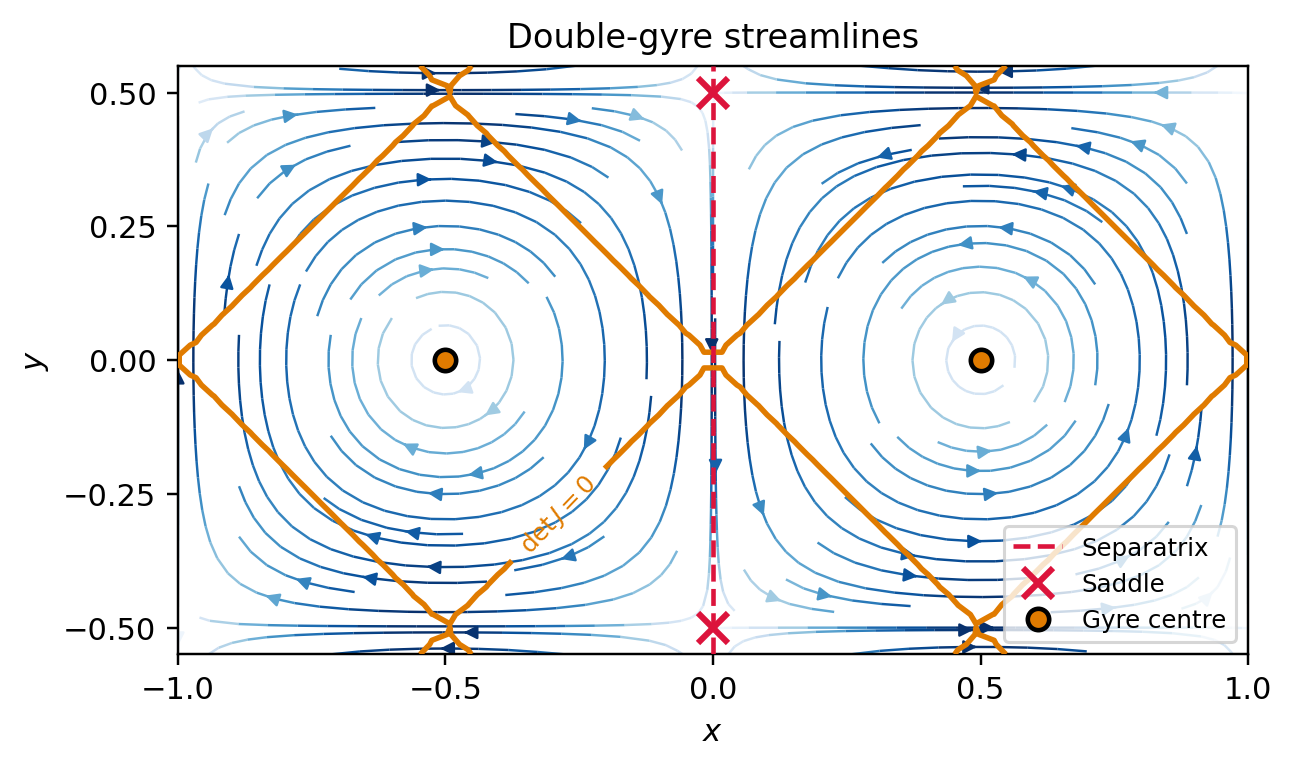
\includegraphics[width=0.45\textwidth]{figures/double_gyre_streamlines.png}
    \caption{Double-gyre vector field (steady case, $A = 0.1$). Streamlines
    are shown in gray. The separatrix at $x = 0$ (dashed) is the stable
    manifold of the lower saddle and the unstable manifold of the upper
    saddle ($\times$). The $D = 0$ Okubo-Weiss boundary (solid) is a
    diamond around each gyre center ($\bullet$).}
    \label{fig:dg_streamlines}
\end{figure}

\begin{figure}[!t]
    \centering
    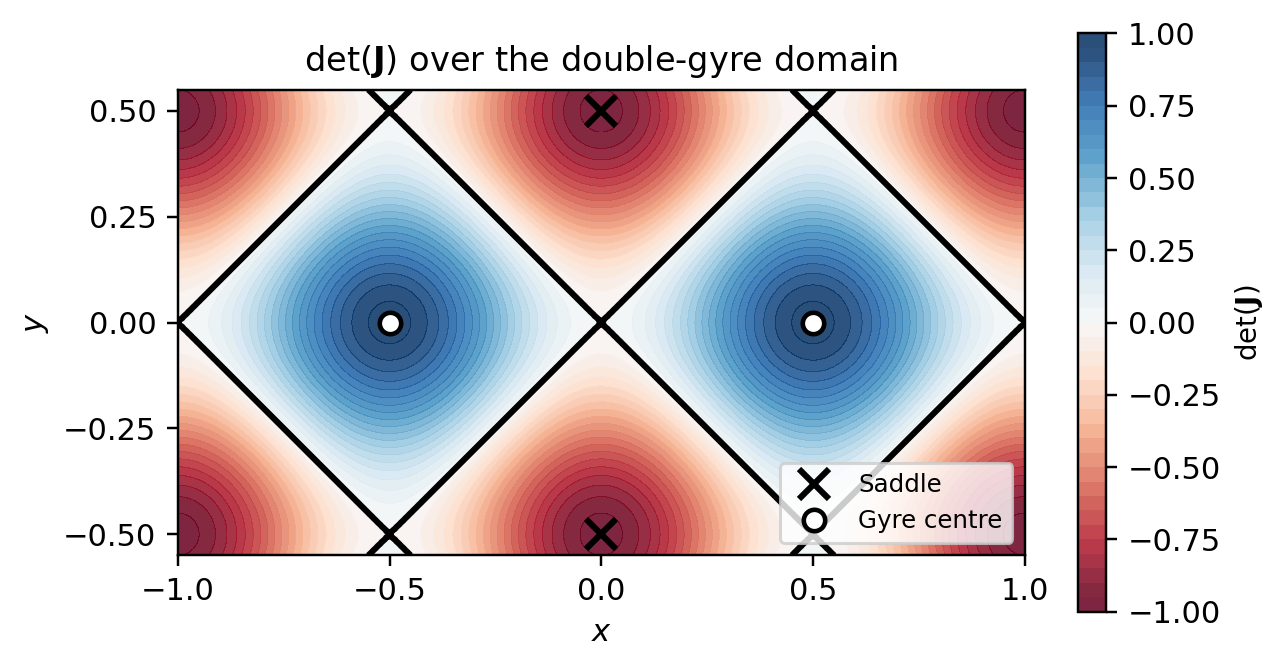
\includegraphics[width=0.45\textwidth]{figures/detJ_contour.png}
    \caption{$D = \det(\mathbf{J})$ over the double-gyre domain. The $D = 0$
    boundary (bold) separates rotation-dominated cores ($D > 0$) from the
    strain-dominated exterior ($D < 0$). The separatrix at $x = 0$ is a
    valley line of $D$ connecting the crest at the origin to the two wells
    at the saddle points.}
    \label{fig:detJ_contour}
\end{figure}

\begin{figure}[!t]
    \centering
    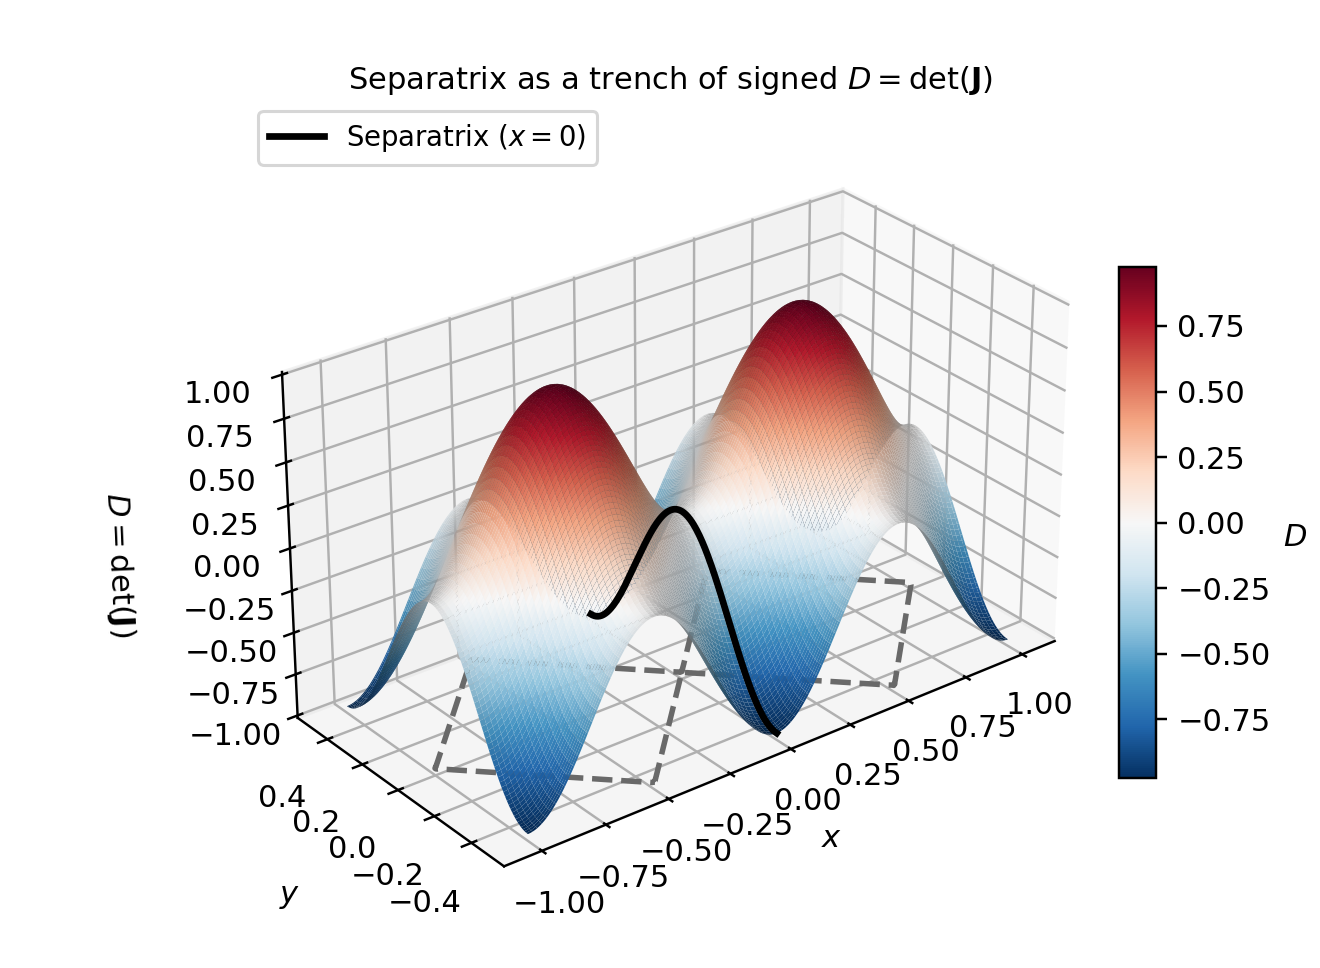
\includegraphics[width=0.45\textwidth]{figures/detJ_trench_cross_section.png}
    \caption{Signed $D = \det(\mathbf{J})$ as an elevation surface over the
    double-gyre domain. The two gyre cores rise as ridges ($D > 0$,
    rotation-dominated) and the exterior falls below zero ($D < 0$,
    strain-dominated); the dashed curve on the floor is the $D = 0$ boundary.
    The separatrix at $x = 0$ (bold) is a valley of $D$ running between the two
    ridges, its floor rising to $D = 0$ at the origin and deepening toward the
    saddle points.}
    \label{fig:trench_cross}
\end{figure}

\subsection{Problem Statement}
\label{sec:problem_statement}

Consider $N$ robots at positions $\mathbf{p}_i$, each measuring the local
flow $(u_i, v_i) = \mathbf{v}(\mathbf{p}_i)$ at the common sampling
instant. No map, forecast, or prior model of the field is available, and
no robot can integrate trajectories of the field. Using only the current
synchronous samples $\{(\mathbf{p}_i, u_i, v_i)\}_{i=1}^{N}$ at each
control cycle, the team must generate a centroid velocity command
$\dot{\mathbf{p}}_c$ that solves:

\emph{Problem (separatrix network traversal).} Drive the cluster
centroid onto the trench of $D$ and travel it, in the direction of the
ambient flow, through the saddle points where trench segments cross.
Terminal capture at a single saddle (Section~\ref{sec:sep_controller}) is
the special case in which the selector's stationary-point test is
tightened to stop the team there instead.

This requires, at minimum, pointwise estimates of $D$, its
gradient $\mathbf{g} = \nabla D$, and its Hessian $\mathbf{H}_D$ at the
centroid. The next section shows how a six-robot formation produces them.


% ---------------------------------------------------------------------------
\section{Distributed Second-Order Estimation}
\label{sec:estimation}

\subsection{Quadratic Fit from Six Simultaneous Measurements}

Let $\tilde{\mathbf{p}}_i = \mathbf{p}_i - \mathbf{p}_c$ denote robot
positions relative to the centroid and define the quadratic basis vector
\begin{equation}
    \boldsymbol{\phi}(\tilde{\mathbf{p}}) =
    \bigl[\,1, \; \tilde{x}, \; \tilde{y}, \; \tfrac{1}{2}\tilde{x}^2, \;
    \tilde{x}\tilde{y}, \; \tfrac{1}{2}\tilde{y}^2\,\bigr]^\top,
    \label{eq:basis}
\end{equation}
whose one-half factors make the fitted coefficients equal to the Taylor
derivatives in (\ref{eq:quad_model_u})--(\ref{eq:quad_model_v}). Stacking
the basis vectors of the six robots row-wise gives the $6 \times 6$
formation matrix $\boldsymbol{\Phi}$, the second-order generalization of
the $3 \times 3$ matrix $\mathbf{A}$ of \cite{14}. The coefficient vectors
$\boldsymbol{\theta}_u = [u_0, u_x, u_y, u_{xx}, u_{xy}, u_{yy}]^\top$ and
$\boldsymbol{\theta}_v = [v_0, v_x, v_y, v_{xx}, v_{xy}, v_{yy}]^\top$
solve the pair of linear systems
\begin{equation}
    \boldsymbol{\Phi}\,\boldsymbol{\theta}_u = \mathbf{u}, \qquad
    \boldsymbol{\Phi}\,\boldsymbol{\theta}_v = \mathbf{v},
    \label{eq:solve}
\end{equation}
where $\mathbf{u} = [u_1, \ldots, u_6]^\top$ and $\mathbf{v} = [v_1,
\ldots, v_6]^\top$ collect the measurements. One matrix factorization
serves both components. When the field is exactly quadratic over the
formation footprint, the solution of (\ref{eq:solve}) is exact for any
nonsingular $\boldsymbol{\Phi}$; for general smooth fields the model
error is quantified in Section~\ref{sec:sensitivity}.

\subsection{Six Robots Are Necessary, and Almost Always Sufficient}

\begin{proposition}[Minimality]
\label{prop:minimality}
Each robot contributes exactly one linear equation to each system in
(\ref{eq:solve}), and each system has six unknowns. Hence no algorithm,
linear or otherwise, can uniquely recover the quadratic model
(\ref{eq:quad_model_u})--(\ref{eq:quad_model_v}) from one synchronous
sample of fewer than six robots, and six robots suffice exactly when
$\boldsymbol{\Phi}$ is nonsingular.
\end{proposition}

\begin{IEEEproof}
With $N < 6$ robots, $\boldsymbol{\Phi} \in \mathbb{R}^{N \times 6}$ has
a nontrivial null space, so for any candidate coefficient vector
$\boldsymbol{\theta}_u$ the vector $\boldsymbol{\theta}_u +
\boldsymbol{\theta}_0$ with $\boldsymbol{\Phi}\boldsymbol{\theta}_0 =
\mathbf{0}$, $\boldsymbol{\theta}_0 \neq \mathbf{0}$, generates identical
measurements at every robot. The two quadratic fields are
indistinguishable from the data, so no estimator can select between
them. With $N = 6$, (\ref{eq:solve}) has a unique solution if and only if
$\det(\boldsymbol{\Phi}) \neq 0$.
\end{IEEEproof}

Nonsingularity has a clean geometric characterization.

\begin{proposition}[Conic criterion]
\label{prop:conic}
$\boldsymbol{\Phi}$ is singular if and only if the six sampling points
lie on a common conic, that is, on the zero set of some nonzero quadratic
polynomial $q(\tilde{x}, \tilde{y})$ (including degenerate conics such as
line pairs).
\end{proposition}

\begin{IEEEproof}
$\boldsymbol{\Phi}$ is singular iff its columns are linearly dependent,
iff there is a nonzero coefficient vector $\mathbf{c}$ with
$\boldsymbol{\phi}(\tilde{\mathbf{p}}_i)^\top \mathbf{c} = 0$ for all
$i$. The function $q = \boldsymbol{\phi}^\top \mathbf{c}$ is precisely a
nonzero polynomial of degree at most two vanishing at all six points.
\end{IEEEproof}

\begin{corollary}[Pentagon plus center]
\label{cor:pentagon}
Place five robots at the vertices of a regular pentagon of radius $\rho$
and the sixth at its center. Then $\boldsymbol{\Phi}$ is nonsingular.
\end{corollary}

\begin{IEEEproof}
No three vertices of a regular pentagon are collinear, and five points in
general position determine a unique conic; for the pentagon vertices that
conic is the circumscribed circle. The center does not lie on the
circle, so no conic passes through all six points, and
Proposition~\ref{prop:conic} applies.
\end{IEEEproof}

\begin{remark}[The center robot is essential]
Any formation whose six robots lie on one circle, for example a regular
hexagon, is singular regardless of its size or orientation, since the
circle itself is a conic through all six points. Rings are natural
formations for mobile robots, which makes this failure mode easy to adopt
by accident; moving one robot to the center removes it entirely.
\end{remark}

\subsection{The Formation and Its Noise Gains}
\label{sec:formation}

The pentagon-plus-center shape is the same minimal configuration that
Bri\~{n}\'{o}n-Arranz et al.\ derived for Hessian estimation of a scalar
field: $N \geq 5$ robots uniformly spaced on a circle plus one at the
center \cite{15}. Their estimator combines the ring measurements with fixed
symmetric weights, which is computationally trivial and, for exactly six
robots on the ideal formation, algebraically equivalent to solving
(\ref{eq:solve}). The two approaches separate when the formation deforms,
as it always does under real formation control: fixed weights assume the
ideal geometry and acquire a bias proportional to the deformation,
whereas (\ref{eq:solve}) uses the measured robot positions and remains
exact for quadratic fields under any deformation short of the conic
degeneracy of Proposition~\ref{prop:conic}. The estimator therefore
degrades gracefully: formation error affects accuracy only through the
conditioning of $\boldsymbol{\Phi}$, which is monitored online through
$\det(\boldsymbol{\Phi})$.

For the ideal formation the noise amplification has closed form. Let each
measurement carry independent zero-mean noise of standard deviation
$\sigma_{uv}$, as in (\ref{eq:meas_noise}). Since
$\hat{\boldsymbol{\theta}}_u - \boldsymbol{\theta}_u =
\boldsymbol{\Phi}^{-1}\boldsymbol{\eta}$, the standard deviation of each
coefficient is $\sigma_{uv}$ times the Euclidean norm of the
corresponding row of $\boldsymbol{\Phi}^{-1}$.

\begin{lemma}[Exact noise gains of the pentagon-plus-center formation]
\label{lem:gains}
For five robots on a ring of radius $\rho$ and one at the centroid, the
coefficient standard deviations are
\begin{equation}
    \sigma_{u_0} = \sigma_{uv}, \quad
    \sigma_{u_x} = \sigma_{u_y} = \frac{2}{\sqrt{10}}\frac{\sigma_{uv}}{\rho},
    \label{eq:gain_grad}
\end{equation}
\begin{equation}
    \sigma_{u_{xx}} = \sigma_{u_{yy}} = \frac{8}{\sqrt{10}}
    \frac{\sigma_{uv}}{\rho^2},
    \qquad
    \sigma_{u_{xy}} = \frac{4}{\sqrt{10}}\frac{\sigma_{uv}}{\rho^2},
    \label{eq:gain_hess}
\end{equation}
independent of the formation heading, and identically for
$\boldsymbol{\theta}_v$.
\end{lemma}

\begin{IEEEproof}
The value coefficient is exact: every basis function except the constant
vanishes at the origin, so interpolation forces $\hat{u}_0$ to equal the
center robot's reading, giving unit gain. The remaining rows follow from
direct inversion of $\boldsymbol{\Phi}$ using the fifth roots of unity;
the row norms reduce to the stated constants, and repeating the
computation with an arbitrary ring phase leaves them unchanged. The
error covariance of the estimated gradient is in fact isotropic,
$\tfrac{4}{10}\sigma_{uv}^2\,\rho^{-2}\mathbf{I}$, for every heading.
\end{IEEEproof}

Two design consequences. First, the gains are isotropic: the error
covariance of the estimated gradient (and of the Hessian, entrywise as
stated) does not depend on the direction of travel, so estimator quality
does not degrade as the cluster turns. Second, the $1/\rho$ and
$1/\rho^2$ factors exhibit the fundamental scaling: second derivatives
are harder to sense than first derivatives by one power of the formation
radius. A numerical search over all six-point formations of the same
footprint found configurations at best a few percent better in worst-case
Hessian gain, so the symmetric shape is used without further tuning.

\begin{figure}[!t]
    \centering
    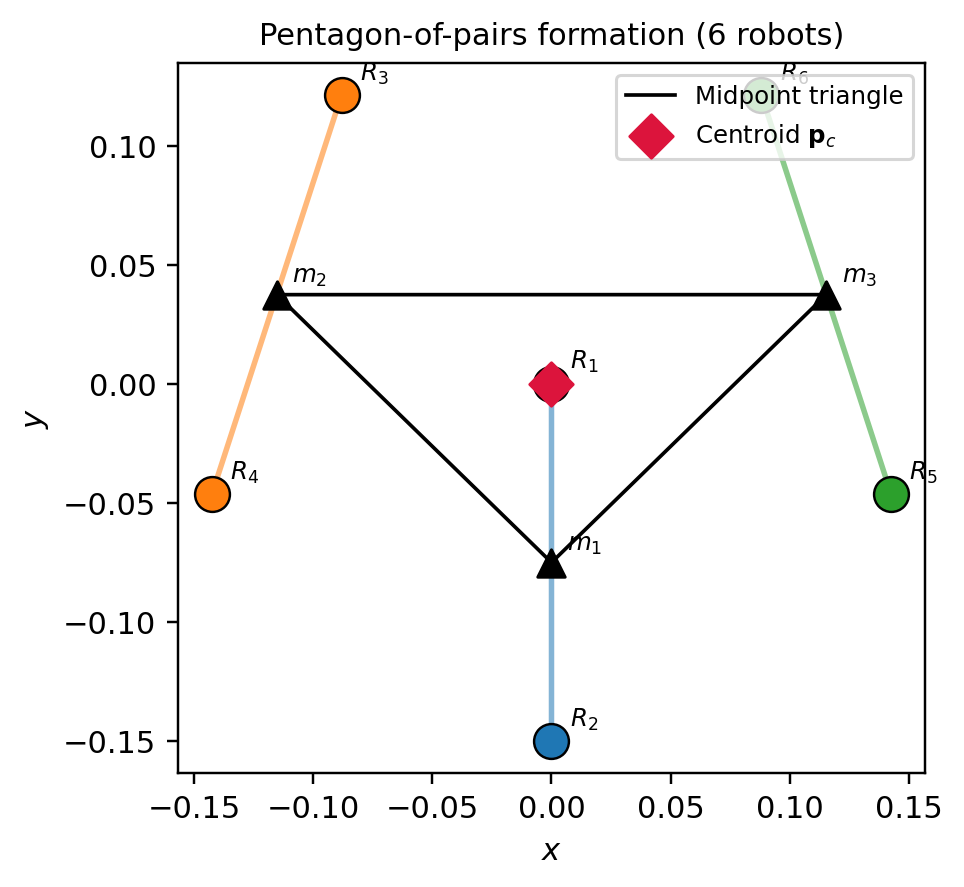
\includegraphics[width=0.40\textwidth]{figures/pentagon_formation.png}
    \caption{Six-robot formation: five robots on a ring of radius $\rho$
    at $72^\circ$ spacing and one robot at the center, the minimal
    symmetric formation for second-order estimation
    (Corollary~\ref{cor:pentagon}, \cite{15}). For formation control the six
    robots are grouped into three pairs whose midpoints define an SAS
    triangle (Appendix~\ref{app:kinematics}); the grouping is invisible to
    the estimator, which uses only the six measured positions.}
    \label{fig:pentagon_formation}
\end{figure}

\subsection{Closed-Form Recovery of $D$, $\nabla D$, and $\mathbf{H}_D$}

The estimated Jacobian at the centroid is assembled from the linear
coefficients,
\begin{equation}
    \hat{\mathbf{J}} =
    \begin{bmatrix} u_x & u_y \\ v_x & v_y \end{bmatrix},
    \qquad
    \hat{D} = u_x v_y - u_y v_x.
    \label{eq:J_hat}
\end{equation}
Under the quadratic model, each entry of $\mathbf{J}$ is an affine
function of position, so $D(\mathbf{p})$ is itself an exactly quadratic
polynomial over the footprint. Its gradient and Hessian at the centroid
are polynomial functions of the fitted coefficients:
\begin{equation}
    \hat{\mathbf{g}} = \nabla \hat{D} =
    \begin{bmatrix}
        u_{xx} v_y + u_x v_{xy} - u_{xy} v_x - u_y v_{xx} \\
        u_{xy} v_y + u_x v_{yy} - u_{yy} v_x - u_y v_{xy}
    \end{bmatrix},
    \label{eq:grad_det}
\end{equation}
\begin{equation}
    \hat{\mathbf{H}}_D =
    \begin{bmatrix}
        2(u_{xx} v_{xy} - u_{xy} v_{xx}) &
        u_{xx} v_{yy} - u_{yy} v_{xx} \\
        u_{xx} v_{yy} - u_{yy} v_{xx} &
        2(u_{xy} v_{yy} - u_{yy} v_{xy})
    \end{bmatrix}.
    \label{eq:hess_det}
\end{equation}
These follow by differentiating $D = u_x v_y - u_y v_x$ with the
third-order terms absent, and require no field evaluations beyond the six
measurements. The omission is harmless for the gradient but not for the
Hessian; its systematic consequences are quantified in
Section~\ref{sec:sensitivity}. The estimated flow at the centroid,
$\mathbf{f} = (u_0, v_0)$, equals the center robot's reading by
Lemma~\ref{lem:gains}. Together
(\ref{eq:J_hat})--(\ref{eq:hess_det}) supply every quantity the
controller of Section~\ref{sec:controllers} consumes: $\hat{D}$,
$\hat{\mathbf{g}}$, $\hat{\mathbf{H}}_D$, and $\mathbf{f}$.

\subsection{Sensitivity: Noise, Truncation, and Formation Radius}
\label{sec:sensitivity}

Three error sources separate cleanly. Write $\boldsymbol{\Phi} =
\bar{\boldsymbol{\Phi}}\,\mathbf{S}_\rho$ with $\mathbf{S}_\rho =
\mathrm{diag}(1, \rho, \rho, \rho^2, \rho^2, \rho^2)$, where
$\bar{\boldsymbol{\Phi}}$ depends only on the formation shape. All
scale dependence enters through $\mathbf{S}_\rho^{-1}$.

\subsubsection{Measurement noise}
By Lemma~\ref{lem:gains}, gradient coefficients degrade as
$\sigma_{uv}/\rho$ and Hessian coefficients as $\sigma_{uv}/\rho^2$:
larger formations average noise better.

\subsubsection{Truncation bias}
If the field is three times differentiable with
$|\partial^3 u|, |\partial^3 v| \leq M_3$ over the footprint, the Taylor
remainder at robot $i$ is bounded by $\tfrac{M_3}{6}\rho^3$, and passing
it through $\mathbf{S}_\rho^{-1}\bar{\boldsymbol{\Phi}}^{-1}$ bounds the
systematic error by
\begin{equation}
    |\hat{u}_x - u_x| \leq c_1 M_3 \rho^2, \qquad
    |\hat{u}_{xx} - u_{xx}| \leq c_2 M_3 \rho,
    \label{eq:truncation}
\end{equation}
and likewise for the remaining coefficients, where $c_1, c_2$ are
absolute constants of the formation shape (row sums of
$|\bar{\boldsymbol{\Phi}}^{-1}|$ divided by six). The Hessian bias decays
only linearly in $\rho$, matching the $O(\rho)$ bound proved for the
symmetric estimator in \cite{15}: smaller formations track curvature better.

\subsubsection{The radius trade-off}
Combining the two effects, the total error of each fitted second-order
coefficient is bounded by
$c_2 M_3 \rho + c_2' \sigma_{uv}/\rho^2$, which is minimized at
\begin{equation}
    \rho^* = \left(\frac{2 c_2' \sigma_{uv}}{c_2 M_3}\right)^{1/3}
    \propto \left(\frac{\sigma_{uv}}{M_3}\right)^{1/3}.
    \label{eq:rho_star}
\end{equation}
The formation radius is thus a sensing parameter, not merely a spacing
choice: it should grow with the noise floor and shrink with the field's
third-derivative scale. This rule is confirmed for $\hat{D}$ and
$\nabla\hat{D}$ by the formation-radius sweeps reported in
Section~\ref{sec:results}; the derived Hessian $\hat{\mathbf{H}}_D$ is
instead limited by the model bias discussed next.

\subsubsection{Propagation to $D$ and its derivatives}
Errors in the fitted coefficients enter the navigation quantities through
products of coefficient pairs. For two-by-two matrices the expansion of
the determinant is exact at second order:
$\det(\mathbf{J} + \mathbf{E}) = \det(\mathbf{J}) +
\operatorname{tr}(\mathrm{adj}(\mathbf{J})\mathbf{E}) + \det(\mathbf{E})$,
and $\|\mathrm{adj}(\mathbf{J})\|_F = \|\mathbf{J}\|_F$, so the estimated
determinant satisfies
\begin{equation}
    |\hat{D} - D| \;\leq\; \|\mathbf{J}\|_F \|\mathbf{E}\|_F
    + \tfrac{1}{2}\|\mathbf{E}\|_F^2,
    \label{eq:det_perturbation}
\end{equation}
where $\mathbf{E} = \hat{\mathbf{J}} - \mathbf{J}$ collects the four
first-order coefficient errors. The gradient formula (\ref{eq:grad_det})
is complete: differentiating $D = u_x v_y - u_y v_x$ once produces only
products of first- and second-order derivatives, so $\hat{\mathbf{g}}$
inherits errors solely from the fitted coefficients, linearly, with
slopes set by the true derivative magnitudes.

The Hessian is different in kind. Differentiating twice produces terms
such as $u_{xxx} v_y$ and $u_y v_{xxx}$, third derivatives of the field
weighted by the field itself, and a quadratic model has no third
derivatives: (\ref{eq:hess_det}) is the Hessian of the fitted quadratic
surface, not of $D$. The omitted terms constitute a model bias that is
independent of the formation radius and cannot be reduced by averaging;
the situation is that of fitting a line to a curved signal and using the
line's slope where the curvature is unmodeled, acceptable exactly where
the model is locally adequate. For the double gyre at the nominal scale
this bias is large in norm, on the order of $\|\mathbf{H}_D\|_F$ itself
(Section~\ref{sec:results}). Two conclusions nevertheless carry into the
stability analysis: the estimate errors entering the controller are
bounded whenever the coefficient errors are bounded, with explicit
formation-dependent constants; and all such constants degrade
continuously, not abruptly, as the formation deforms, with outright
failure only on the conic configurations of
Proposition~\ref{prop:conic}.

\begin{remark}[What survives the Hessian bias]
\label{rem:eigvec}
The controller of Section~\ref{sec:controllers} consumes
$\hat{\mathbf{H}}_D$ only through its eigenvectors and the signs and
rough magnitudes of its eigenvalues, and these degrade far less than the
Frobenius error suggests. The double gyre is symmetric under reflection
across the separatrix, so $D$ is even in the transverse coordinate and
every odd transverse derivative, including the mixed second derivative,
vanishes on the trench: both the retained and the omitted terms are
diagonal in the trench frame there. The estimated eigen-directions on
the separatrix are exact to numerical precision, remain within a few
tenths of a degree across the tube, and within a few degrees at generic
points (Section~\ref{sec:results}), while the bias loads almost entirely
onto the eigenvalues. The transverse Newton snap divides the transverse
gradient by the transverse eigenvalue, so an eigenvalue bias rescales
the step, which the saturation (\ref{eq:sat}) bounds and the closed loop
absorbs; it does not rotate the commanded direction. This is why a
formation too small to sense curvature accurately can still track the
structure that curvature defines. The exception is the immediate
neighborhood of the wells, where the biased eigenvalues nearly vanish
and their signs become unreliable; the consequences for terminal capture
are examined in Section~\ref{sec:results}.
\end{remark}


% ---------------------------------------------------------------------------
\section{Adaptive Navigation Controllers}
\label{sec:controllers}

\subsection{Control Architecture}
\label{sec:arch}

The controller runs inside the three-layer architecture of \cite{14,30}:

\begin{enumerate}
    \item \textbf{Navigation primitive.} From the six positions and
          measurements, compute the estimates
          (\ref{eq:J_hat})--(\ref{eq:hess_det}) and output a centroid
          velocity command $\dot{\mathbf{p}}_c^{\,\text{des}}$.
    \item \textbf{Cluster space controller.} Using the twelve-state
          cluster parameterization and its analytic inverse kinematic
          Jacobian (Appendix~\ref{app:kinematics}), distribute the
          centroid command to six robot velocity commands while
          regulating the formation shape to its nominal geometry.
    \item \textbf{Robot dynamics.} Each robot obeys the first-order
          momentum model identified on the Decabot hardware \cite{14},
          \begin{equation}
              \mathbf{v}[k+1] = \alpha_{\text{mom}}\,\mathbf{v}[k]
              + (1 - \alpha_{\text{mom}})\,\mathbf{v}^{\text{des}}[k],
              \label{eq:momentum}
          \end{equation}
          with $\alpha_{\text{mom}} = \exp(-\Delta t/\tau)$, actuator
          time constant $\tau = 0.3$ s, control period $\Delta t = 0.1$ s
          (so $\alpha_{\text{mom}} \approx 0.717$), speed limit
          $v_{\text{max,robot}} = 0.3$ m/s, and stiction floor
          $v_{\text{stiction}} = 0.025$ m/s.
          % 0.05 m/s was the three-robot paper's value; the six-robot
          % simulation uses the Omnibot default 0.025 (omnibot.py).
\end{enumerate}

Note on notation: $\alpha_{\text{mom}}$ in (\ref{eq:momentum}) is the
momentum coefficient of the robot model; it is unrelated to
$\alpha_{\text{eig}}$, the real part of a complex eigenvalue pair of
$\mathbf{J}$ used in field classification.

\subsection{From the Newton Step to the Modified Newton Step}
\label{sec:mod_newton}

Under the quadratic model, $\hat{D}(\mathbf{p})$ is an exact quadratic
surface with gradient $\hat{\mathbf{g}}$ and constant Hessian
$\hat{\mathbf{H}}_D$ at the centroid, so the natural navigation move is
the Newton step $\Delta\mathbf{p} = -\hat{\mathbf{H}}_D^{-1}
\hat{\mathbf{g}}$, which jumps to the stationary point of the local
model in one move. Written in the eigenbasis
$\hat{\mathbf{H}}_D \mathbf{w}_k = \lambda_k \mathbf{w}_k$, with
$\lambda_1 \leq \lambda_2$ throughout, the step decomposes into
per-direction components $-(\mathbf{w}_k^\top
\hat{\mathbf{g}})/\lambda_k$. Two defects make the raw step unsuitable
as a velocity command, and each is repaired by one modification.

First, the magnitude is unbounded and explodes where
$\hat{\mathbf{H}}_D$ is near singular. The repair is componentwise
saturation through
\begin{equation}
    \mathrm{sat}(c) = v_{\max} \tanh\!\left(\frac{c}{v_{\max}}\right),
    \label{eq:sat}
\end{equation}
which gives a bounded constant-speed reach far from the structure and
recovers the exact Newton component, with its superlinear local
convergence, once $|c| \ll v_{\max}$. A single parameter $v_{\max}$
sets both the cruise speed and the width of the terminal boundary
layer. The saturated Newton step is the \emph{attract step},
\begin{equation}
    \dot{\mathbf{p}}_c^{\,\text{des}} = \sum_{k=1}^{2}
    \mathrm{sat}\!\left(-\frac{\mathbf{w}_k^\top
    \hat{\mathbf{g}}}{\lambda_k}\right)\mathbf{w}_k.
    \label{eq:attract_step}
\end{equation}

Second, and more fundamentally, (\ref{eq:attract_step}) converges to
whatever stationary point the local model exhibits, with no preference
among minima, maxima, and saddle points of $D$. On a trench the
along-trench curvature can be negative (the crest side), and there the
Newton component deliberately climbs. The modification, adopted from
saddle-free Newton methods in optimization \cite{35}, replaces the signed
eigenvalue by its magnitude, giving the \emph{slide step},
\begin{equation}
    \dot{\mathbf{p}}_c^{\,\text{des}} = \sum_{k=1}^{2}
    \mathrm{sat}\!\left(-\frac{\mathbf{w}_k^\top
    \hat{\mathbf{g}}}{|\lambda_k|}\right)\mathbf{w}_k.
    \label{eq:slide_step}
\end{equation}
In directions of positive curvature the two laws agree and snap the
centroid onto the trench floor; in the direction of negative curvature
(\ref{eq:slide_step}) reverses the Newton component into a
curvature-normalized descent that slides along the trench, away from
crests. Both laws are well defined despite the sign ambiguity of
eigenvectors: every term is quadratic in $\mathbf{w}_k$, so replacing
$\mathbf{w}_k$ by $-\mathbf{w}_k$ leaves the command unchanged.

\subsection{Separatrix Tracker}
\label{sec:sep_controller}

The separatrix tracker composes the two step bodies with a third,
flow-assisted mode. The need for the third mode is visible in the trench
profile of Section~\ref{sec:dg_example}: the slide step descends $D$
along the trench, but at the crest the along-trench gradient vanishes,
and on the upstream side of the crest descent points away from the flow
direction, while the separatrix continues through the crest. On the
separatrix itself, however, the ambient flow is tangent to the structure
and nonzero away from the saddles, so the flow can carry the team across
the crest. The cluster is declared on the separatrix
(FLOW band) when either
\begin{equation}
    |\hat{D}| < \varepsilon_{\text{raw}}
    \quad\text{or}\quad
    \frac{|\hat{D}|}{\|\hat{\mathbf{H}}_D\|_F} < \varepsilon_{\text{dim}},
    \label{eq:flow_band}
\end{equation}
where $\varepsilon_{\text{raw}}$ is a raw threshold and
$\varepsilon_{\text{dim}}$ a curvature-normalized threshold (units of
length squared) that makes the band scale with the local landscape. In
the FLOW band the command follows the measured flow along the trench
tangent $\mathbf{w}_1$ and retains the Newton snap across it: the
\emph{flow step} is
\begin{equation}
    \dot{\mathbf{p}}_c^{\,\text{des}} =
    \mathrm{sat}\!\left(\mathbf{f}^\top \mathbf{w}_1\right)\mathbf{w}_1
    + \mathrm{sat}\!\left(-\frac{\hat{\mathbf{g}}^\top
    \mathbf{w}_2}{\lambda_2}\right)\mathbf{w}_2.
    \label{eq:flow_step}
\end{equation}
Off the band, the local flow direction selects between the attract and
slide laws: if the flow agrees with the along-trench descent direction
the team slides (\ref{eq:slide_step}); if it opposes descent the team
attracts toward the local stationary point (\ref{eq:attract_step}),
which lies at the crest, inside the FLOW band, so the attract law hands
the team over to the flow. In all three modes the tangential motion is
never directed against the ambient flow, a fact used in the stability
analysis. The complete selector, executed once per control cycle after
the estimation step, is:

\vspace{4pt}
\hrule
\vspace{4pt}
\noindent\textbf{Separatrix tracker: one control cycle}

\vspace{3pt}
\noindent\textbf{Parameters:} $v_{\max}$, $\varepsilon_{\text{raw}}$,
$\varepsilon_{\text{dim}}$\\
\textbf{Given:} $\hat{D}$, $\hat{\mathbf{g}}$, $\hat{\mathbf{H}}_D$,
$\mathbf{f}$ from (\ref{eq:J_hat})--(\ref{eq:hess_det}), and eigenpairs
$(\lambda_1, \mathbf{w}_1)$, $(\lambda_2, \mathbf{w}_2)$ of
$\hat{\mathbf{H}}_D$, $\lambda_1 \leq \lambda_2$

\vspace{3pt}
\noindent If the band test (\ref{eq:flow_band}) passes (on the
separatrix):\\
\hspace*{1.5em} apply the flow step (\ref{eq:flow_step}).\\
Else, if $\lambda_1 \lambda_2 \geq 0$ ($\hat{D}$ has no saddle; near a
well of $D$):\\
\hspace*{1.5em} apply the attract step (\ref{eq:attract_step}).\\
Else, orient $\mathbf{w}_1$ so that $\hat{\mathbf{g}}^\top \mathbf{w}_1
\leq 0$ (descent along the trench):\\
\hspace*{1.5em} if $\mathbf{f}^\top \mathbf{w}_1 > 0$ (flow agrees with
descent), apply the slide step (\ref{eq:slide_step});\\
\hspace*{1.5em} otherwise (flow opposes descent), apply the attract
step (\ref{eq:attract_step}).
\vspace{4pt}
\hrule
\vspace{4pt}

The implementation is \textit{separatrix\_logic\_c\_step} in
\textit{pentagon\_primitives.py}. Note that the $\mathbf{w}_2$
component is one and the same in all three laws
(\ref{eq:attract_step}), (\ref{eq:slide_step}), and
(\ref{eq:flow_step}): on a trench, $\lambda_2 > 0$, so the signed and
magnitude denominators agree, and every mode applies the identical
transverse Newton snap. The modes differ only in their motion along the
structure. This shared component is what makes the switched system
tractable in Section~\ref{sec:stability}.

\subsection{Gains and Velocity Limits}

The controller saturates every component through $v_{\max}\tanh(c /
v_{\max})$, so the commanded centroid speed never exceeds
$\sqrt{2}\,v_{\max}$. The primitive-level saturation speed is $v_{\max}
= 0.04$ m/s, amplified by a fixed navigation gain $k = 3$ before the
cluster layer so that steady commands clear the robots' stiction floor;
the robot-level limits of (\ref{eq:momentum}) are unchanged from \cite{14}.
The band thresholds $\varepsilon_{\text{raw}} = 10^{-3}$ and
$\varepsilon_{\text{dim}} = 0.025$ are fixed in all experiments unless
noted.

Table~\ref{tab:params} collects the values used in all experiments.

\begin{table}[!t]
\centering
\caption{Simulation and controller parameters}
\label{tab:params}
\footnotesize
\setlength{\tabcolsep}{4pt}
\begin{tabular}{llll}
\hline
\textbf{Symbol} & \textbf{Value} & \textbf{Units} & \textbf{Description} \\
\hline
$v_{\max}$ & 0.04 & m/s & primitive saturation speed \\
$k$ & 3.0 & -- & navigation gain \\
$v_{\text{max,robot}}$ & 0.3 & m/s & robot speed limit \\
$v_{\text{stiction}}$ & 0.025 & m/s & robot stiction floor \\
$\tau$ & 0.3 & s & actuator time constant \\
$\Delta t$ & 0.1 & s & control period \\
$\alpha_{\text{mom}}$ & 0.717 & -- & momentum coefficient $e^{-\Delta t/\tau}$ \\
$A$ & 0.1 & -- & double-gyre amplitude \\
$\rho$ & 0.075 & m & formation ring radius \\
$\varepsilon_{\text{raw}}$ & $10^{-3}$ & s$^{-2}$ & FLOW-band raw threshold \\
$\varepsilon_{\text{dim}}$ & 0.025 & m$^{2}$ & FLOW-band dimensionless threshold \\
\hline
\end{tabular}
\end{table}


% ---------------------------------------------------------------------------
\section{Stability Analysis}
\label{sec:stability}

\subsection{Closed-Loop Model and Standing Assumptions}

The analysis is carried out at the navigation level: the cluster
centroid is modeled as a kinematic integrator
\begin{equation}
    \dot{\mathbf{p}}_c = k\,\boldsymbol{\delta}(\mathbf{p}_c),
    \label{eq:kinematic_model}
\end{equation}
where $\boldsymbol{\delta}$ is the output of the separatrix tracker,
and $k > 0$ is the navigation gain. This abstracts the cluster and
robot layers, whose
tracking dynamics (\ref{eq:momentum}) are faster than the navigation
timescale ($\tau = 0.3$ s against transit times of tens of seconds);
the same separation was validated in hardware in \cite{14}. Time is rescaled
so that $k = 1$. Unless stated otherwise the estimates are taken exact
($\hat{D} = D$, $\hat{\mathbf{g}} = \mathbf{g}$, $\hat{\mathbf{H}}_D =
\mathbf{H}_D$, $\mathbf{f} = \mathbf{v}(\mathbf{p}_c)$);
Section~\ref{sec:stab_iss} restores bounded estimation error.
Throughout, $\mathbf{w}_1, \mathbf{w}_2$ denote unit eigenvectors of
$\mathbf{H}_D$ with $\lambda_1 \leq \lambda_2$, and $z_k =
(\mathbf{w}_k^\top \mathbf{g})/\lambda_k$ the Newton components, so
that the attract step (\ref{eq:attract_step}) reads
$\boldsymbol{\delta} = -\sum_k \mathrm{sat}(z_k)\,\mathbf{w}_k$.

\subsection{The Attract Mode Is a Gradient-Norm Descent}

The first result needs no trench structure at all: it certifies the attract step
globally, wherever $\mathbf{H}_D$ is nonsingular.

\begin{theorem}[Attract-mode certificate]
\label{thm:attract}
Let $V_A = \tfrac{1}{2}\|\mathbf{g}(\mathbf{p}_c)\|^2$. Along
(\ref{eq:kinematic_model}) with the attract step
(\ref{eq:attract_step}),
\begin{equation}
    \dot{V}_A = -v_{\max} \sum_{k=1}^{2} \lambda_k^2\,
    z_k \tanh\!\left(\frac{z_k}{v_{\max}}\right) \;\leq\; 0,
    \label{eq:VA_dot}
\end{equation}
with equality exactly where $\mathbf{g} = \mathbf{0}$. Consequently
every bounded trajectory on which $\mathbf{H}_D$ remains nonsingular
converges to the critical set $\{\mathbf{g} = \mathbf{0}\}$ of $D$, and
isolated critical points with $\mathbf{H}_D$ nonsingular are locally
exponentially stable.
\end{theorem}

\begin{IEEEproof}
Since $\nabla V_A = \mathbf{H}_D \mathbf{g}$,
$\dot{V}_A = \mathbf{g}^\top \mathbf{H}_D \boldsymbol{\delta}
= -\sum_k v_{\max} \tanh(z_k/v_{\max})\,
\mathbf{g}^\top \mathbf{H}_D \mathbf{w}_k
= -\sum_k v_{\max} \tanh(z_k/v_{\max})\,\lambda_k
(\mathbf{w}_k^\top\mathbf{g})$, and $\lambda_k(\mathbf{w}_k^\top
\mathbf{g}) = \lambda_k^2 z_k$, giving (\ref{eq:VA_dot}); each summand
is nonnegative because $z\tanh z \geq 0$. Equality requires $z_1 = z_2 =
0$, that is $\mathbf{g} = \mathbf{0}$. Convergence to the critical set
follows from the invariance principle. Near an isolated critical point
$|z_k| \ll v_{\max}$, the saturation is inactive at first order,
$\boldsymbol{\delta} \approx -\mathbf{H}_D^{-1}\mathbf{g} \approx
-(\mathbf{p}_c - \mathbf{p}^\star_D)$, a unit-rate linear contraction.
\end{IEEEproof}

Theorem~\ref{thm:attract} explains the two roles the attract step plays
in the selector. Far from the trench it provides the approach: it descends
$\|\nabla D\|^2$ toward the stationary set of $D$, which for the double
gyre consists of the trench line's crest and wells and the gyre
centers. Near a well of $D$, where $\mathbf{H}_D \succ 0$, it is the
terminal capture law: the well is the saddle point of the flow, and
convergence is exponential.

\subsection{Separatrix Tracker}
\label{sec:stab_sep}

The trench is formalized as a valley line. The double gyre satisfies all
of the following exactly, with the constants given below.

\begin{assumption}[Nondegenerate straight trench]
\label{ass:trench}
There is a segment $\Gamma$ (take it along the unit vector
$\hat{\mathbf{e}}_\parallel$, with normal $\hat{\mathbf{e}}_\perp$, and
coordinates $(s, n)$) and a tube $T_w = \{|n| \leq w\}$ on which
\begin{equation}
    D(s, n) = \varphi(s) + \tfrac{1}{2}\lambda_\perp(s)\,n^2,
    \qquad 0 < \underline{\lambda} \leq \lambda_\perp(s),
    \label{eq:normal_form}
\end{equation}
the cross terms vanish
($\hat{\mathbf{e}}_\perp^\top \mathbf{H}_D \hat{\mathbf{e}}_\parallel
= 0$ on $T_w$), and on $T_w$ the eigenvalue gap satisfies
$\lambda_2 - \lambda_1 \geq \gamma > 0$ wherever the selector is
outside its attract fallback. For the double gyre separatrix,
(\ref{eq:normal_form}) holds with $n = x$, $s = y$, $\varphi(s) =
-\tfrac{\pi^4 A^2}{2}(1 + \cos 2\pi s_f)$ exactly (the field
(\ref{eq:det_analytic_main}) is additively separable), and
$\lambda_\perp = 2\pi^6 A^2 \cos 2\pi x_f \geq \underline{\lambda}$ on
any tube with $w < 1/4$.
\end{assumption}

\begin{assumption}[Flow structure on the trench]
\label{ass:flow}
$\Gamma$ is an invariant curve of the flow: $\mathbf{v}$ restricted to
$\Gamma$ is tangent to it, with $\|\mathbf{v}\| \geq f_{\min} > 0$
outside balls of radius $r_0$ around the flow saddles, where the flow
vanishes. Along $\Gamma$, the stationary points of $\varphi$ are of two
kinds only: wells located at the flow saddles, and crests located inside
the FLOW band (\ref{eq:flow_band}); quantitatively, $|\varphi'(s)| \geq
m_\varphi > 0$ wherever the band condition fails on $\Gamma$.
\end{assumption}

\begin{lemma}[Common transverse contraction]
\label{lem:transverse}
Under Assumption~\ref{ass:trench}, in every mode of the separatrix
tracker the transverse coordinate obeys
\begin{equation}
    \dot{n} = -v_{\max}\tanh\!\left(\frac{n}{v_{\max}}\right),
    \label{eq:n_dynamics}
\end{equation}
so $|n|$ decreases strictly for $n \neq 0$, the tube $T_w$ is forward
invariant, and $n \to 0$ exponentially once $|n| \leq v_{\max}$. In
particular (\ref{eq:n_dynamics}) is unaffected by arbitrary switching
among the three modes.
\end{lemma}

\begin{IEEEproof}
By (\ref{eq:normal_form}) the Hessian is diagonal in
$(\hat{\mathbf{e}}_\parallel, \hat{\mathbf{e}}_\perp)$ with transverse
eigenvalue $\lambda_\perp > 0$ and eigenvector
$\hat{\mathbf{e}}_\perp$, and the transverse gradient component is
$\hat{\mathbf{e}}_\perp^\top \mathbf{g} = \lambda_\perp n$. The
$\hat{\mathbf{e}}_\perp$ component of the attract step
(\ref{eq:attract_step}), of the slide step (\ref{eq:slide_step}) (the
transverse eigenvalue is positive, so the signed and magnitude
denominators agree), and of the flow step (\ref{eq:flow_step}) are all
built from the same argument $-\lambda_\perp n / \lambda_\perp = -n$.
Saturation gives (\ref{eq:n_dynamics}). The right side is negative for $n > 0$ and
positive for $n < 0$, so $V_\perp = \tfrac{1}{2}n^2$ is a common
Lyapunov function for the switched system; for $|n| \leq v_{\max}$,
$\tanh(n/v_{\max}) \geq n \tanh(1)/v_{\max}$ yields $\dot{V}_\perp \leq
-2\tanh(1) V_\perp$.
\end{IEEEproof}

\begin{lemma}[Flow-consistent progress]
\label{lem:progress}
Under Assumptions~\ref{ass:trench} and \ref{ass:flow}, on $\Gamma$
(after the transient of Lemma~\ref{lem:transverse}) the tangential
velocity component $\dot{s}$ satisfies, in every mode,
$\dot{s}\,(\mathbf{v}^\top \hat{\mathbf{e}}_\parallel) \geq 0$: the team
never moves against the ambient flow along the trench. Moreover
$|\dot{s}| \geq m > 0$ outside the $r_0$ balls, with
\begin{equation}
    m = \min\Bigl\{
    v_{\max}\tanh\!\bigl(\tfrac{f_{\min}}{v_{\max}}\bigr),\;
    v_{\max}\tanh\!\bigl(\tfrac{m_\varphi}
    {\bar{\lambda}_\parallel v_{\max}}\bigr)
    \Bigr\},
    \label{eq:progress_rate}
\end{equation}
where $\bar{\lambda}_\parallel$ bounds $|\lambda_1|$ on the tube.
\end{lemma}

\begin{IEEEproof}
On $\Gamma$ the tangential gradient component is $\varphi'(s)$ and the
along-trench eigenvector is $\hat{\mathbf{e}}_\parallel$. In the FLOW band
the tangential command is $v_{\max}\tanh((\mathbf{f}^\top
\mathbf{w}_1)/v_{\max})$ applied along $\mathbf{w}_1 = \pm
\hat{\mathbf{e}}_\parallel$; the product form makes it a nonnegative
multiple of the flow's tangential component, and by
Assumption~\ref{ass:flow} the crest region is covered by this mode, with
magnitude at least the first argument of (\ref{eq:progress_rate}). Off
the band, the slide step is selected precisely when the flow agrees with the
descent direction $-\mathrm{sign}(\varphi')\hat{\mathbf{e}}_\parallel$,
and its tangential command moves along descent with magnitude
$v_{\max}\tanh(|\varphi'|/(|\lambda_1| v_{\max}))$; the attract step is selected
when the flow opposes descent, and its tangential command,
$-\varphi'/\lambda_1$ with $\lambda_1 < 0$, moves along ascent, which by
the selector's own condition is again the flow direction, with the same
magnitude. In the attract fallback ($\mathbf{H}_D \succeq 0$ near the
wells) the tangential command descends toward the well, which is the
flow direction near a stable-manifold endpoint. In all cases the sign
agrees with the flow and the magnitude is bounded below by
(\ref{eq:progress_rate}) via Assumption~\ref{ass:flow}.
\end{IEEEproof}

\begin{theorem}[Separatrix network traversal]
\label{thm:separatrix}
Under Assumptions~\ref{ass:trench} and \ref{ass:flow}, with exact
estimates, every trajectory of the separatrix tracker starting in the
tube $T_w$
(i) remains in $T_w$ and converges exponentially to the trench, and (ii)
traverses the trench in the direction of the ambient flow, reaching the
$r_0$ neighborhood of a flow saddle in finite time bounded by
$L_\Gamma/m$ with $L_\Gamma$ the trench length. At the saddle, $D$
attains a local minimum with $\mathbf{H}_D \succ 0$
($\mathbf{H}_D = 2\pi^6 A^2\,\mathbf{I}$ at the double-gyre saddles), so
the selector's stationary-point test $\lambda_1\lambda_2 \geq 0$
(Section~\ref{sec:sep_controller}) is satisfied there and (iii)
Theorem~\ref{thm:attract} gives local exponential convergence to the
saddle, terminal capture, exactly as stated. The trench, however, is not
a single arc: Section~\ref{sec:dg_example} shows the saddle is a
crossing of two trench segments running perpendicular to one another. A
selector that reaches the ball and does not satisfy the stationary-point
test, because its estimate of $\mathbf{H}_D$ fails to certify positive
definiteness there, remains in the FLOW or SLIDE modes of
Assumption~\ref{ass:flow} and continues onto the crossing segment
instead of capturing, repeating (i)-(ii) with $\Gamma$ now the new
segment. Capture and continuation are the same theorem applied to
different premises at the crossing; which one the physical controller
exhibits is an estimation question, addressed next.
\end{theorem}

\begin{IEEEproof}
(i) is Lemma~\ref{lem:transverse}. (ii): by Lemma~\ref{lem:progress},
$s(t)$ is monotone in the flow direction with rate at least $m$ outside
the $r_0$ balls, and mode switches cannot reverse it, so the ball is
reached in time at most $L_\Gamma/m$. Capture (iii): inside the ball,
$\mathbf{H}_D \succ 0$, the selector is in its attract fallback, and
Theorem~\ref{thm:attract} gives local exponential convergence to the
well, which coincides with the flow saddle $\mathbf{p}^*$. Continuation:
if the fallback test fails to trigger despite $\mathbf{H}_D \succ 0$
holding for the true field, the selector instead falls through to
Lemma~\ref{lem:progress}'s flow or descent case on whichever of the two
crossing segments the flow direction and sign convention of
$\hat{\mathbf{g}}$ select, and (i)-(ii) apply unchanged with $\Gamma$
relabeled.
\end{IEEEproof}

\begin{remark}[Role of each mode]
The proof assigns each mode a precise job: the transverse Newton snap
(common to all modes) makes the trench attractive; the slide step produces the
descent along the trench; the flow step carries the team across the crest, where
descent is undefined; the attract step turns upstream starts around by climbing to
the crest, and, when its stationary-point test fires at a well, doubles as the
terminal capture law. The
hybrid has no chattering issue in the transverse channel because all
modes share the dynamics (\ref{eq:n_dynamics}).
\end{remark}

\begin{remark}[Capture depends on an estimated, not exact, Hessian]
\label{rem:capture_gap}
Theorem~\ref{thm:separatrix} is stated for exact estimates, under which
$\mathbf{H}_D \succ 0$ at the saddle is certified and capture occurs.
Remark~\ref{rem:eigvec} identifies exactly where this fails for the
closed-form estimator: near the wells the biased eigenvalues nearly
vanish and their signs become unreliable, so the stationary-point test
does not fire on $\hat{\mathbf{H}}_D$ even without noise, and the
selector takes the continuation branch of the proof rather than the
capture branch. Section~\ref{sec:results} confirms this is what the
simulated controller does at every saddle it reaches. Terminal capture
is recovered by tightening the test the selector uses, demonstrated as
a one-parameter alternative in Section~\ref{sec:discussion}; both
behaviors are consequences of the same theorem, differing only in which
premise the deployed estimator satisfies at the crossing.
\end{remark}

\subsection{Robustness to Estimation Error}
\label{sec:stab_iss}

Finally the exact-estimate assumption is dropped. By
Section~\ref{sec:sensitivity}, noise of level $\sigma_{uv}$ and
truncation over a footprint of radius $\rho$ perturb every quantity the
controller uses; the perturbations are bounded, with constants
determined by the formation. Their effect enters each control channel
inside a $\tanh$, which is 1-Lipschitz, so a perturbation of a
commanded component is no larger than the perturbation of its argument.

\begin{proposition}[Ultimate bound under bounded estimate error]
\label{prop:iss}
Suppose the estimate errors induce a bounded disturbance $d(t)$, $|d|
\leq \bar{d} < v_{\max}$, in the transverse channel, so that
(\ref{eq:n_dynamics}) becomes $\dot{n} = -v_{\max}\tanh(n/v_{\max}) +
d$. Then the trench remains practically stable with ultimate bound
\begin{equation}
    \limsup_{t\to\infty} |n(t)| \;\leq\;
    v_{\max}\operatorname{artanh}\!\left(\frac{\bar{d}}{v_{\max}}\right),
    \label{eq:iss_bound}
\end{equation}
which is $\approx \bar{d}$ for $\bar{d} \ll v_{\max}$.
\end{proposition}

\begin{IEEEproof}
$\tfrac{d}{dt}\tfrac{1}{2}n^2 = n(-v_{\max}
\tanh(n/v_{\max}) + d) < 0$ whenever $v_{\max}\tanh(|n|/v_{\max}) >
\bar{d}$, that is outside the stated interval, which is therefore
attractive and invariant.
\end{IEEEproof}

The disturbance level $\bar{d}$ inherits the structure
of Section~\ref{sec:sensitivity}: a noise part scaling as
$\sigma_{uv}/\rho$ to $\sigma_{uv}/\rho^2$ through Lemma~\ref{lem:gains}
and (\ref{eq:det_perturbation}), and a truncation part scaling as
$M_3\rho$ to $M_3\rho^2$ through (\ref{eq:truncation}). The ultimate
bound (\ref{eq:iss_bound}) therefore
degrades linearly in the measurement noise level, with the formation
radius trading the two contributions as in (\ref{eq:rho_star}). The
Monte Carlo sweep of Section~\ref{sec:test_plan} quantifies these
predictions empirically.


% ---------------------------------------------------------------------------
\section{Simulation and Analysis}
\label{sec:methods}

\subsection{Cluster Space Controller and Pentagon Formation}

The controller uses a cluster space controller and pentagon-of-pairs
formation. The forward kinematics maps the 12-state
cluster configuration to global robot positions; the inverse kinematics
and analytic $12 \times 12$ inverse kinematic Jacobian (see
Appendix~\ref{app:kinematics}) map a desired centroid velocity to
individual robot velocity commands while maintaining nominal pair lengths
and the SAS shape of the midpoint triangle.

Formation maintenance is proportional: each of the nine shape-error
terms in $(p_1, \beta_1, q_1, L_2, \psi_2, L_3, \psi_3, L_4, \psi_4)$ is
driven toward its nominal value at a rate proportional to its current
error, with gain $1.0$ on the length terms and $0.1$ on the angle terms
(\textit{position\_gain}, \textit{angle\_gain} in
\textit{pentagon\_cluster.py}), fixed across all experiments.

\subsection{Six-Robot Configuration}

All simulation trials use the same nominal formation
(\textit{pentagon\_small.yaml}), the pentagon-of-pairs of
Appendix~\ref{app:kinematics} at $0.5\times$ its base scale: midpoint
triangle $p_1 = 0.0806$, $\beta_1 = 0.7726$~rad, $q_1 = 0.1154$; pair
lengths $L_2 = 0.0750$, $L_3 = L_4 = 0.0882$; base pair orientations
$\psi_2 = -\pi/2$, $\psi_3 = -1.885$, $\psi_4 = 1.885$~rad and base
heading $\theta_c = -0.7726$~rad. A trial's initial heading is applied
as a rigid rotation of this base configuration by a single offset
angle, so the formation's shape is fixed and only its orientation
varies across trials. This gives the ring radius $\rho = 0.075$ used
throughout Section~\ref{sec:sensitivity} and Table~\ref{tab:params}.
The centroid $(x_c, y_c)$ is placed at the trial's start point
(Section~\ref{sec:test_plan}); the heading offset is drawn uniformly
from $[0, 2\pi)$ per trial in the Monte Carlo sweeps and left at zero
(the base orientation above) in the clean, noise-free demonstration
runs of Section~\ref{sec:results}.

\subsection{Simulation Program}

Simulations are run using the Python framework in the
\textit{trunk/Python\_Simulations/Vector\_Fields/VF\_Robot/} directory.
% Entry points: experiments/separatrix_clean_runs.py, ow_clean_runs.py,
% park_vs_traverse_demo.py, mc_sweep_separatrix.py, mc_sweep_ow.py,
% estimator_accuracy_sweep.py, main_ocean_hfr_2km_ftle_overlay.py,
% ocean_hfr_2km_panel_progression.py, ocean_hfr_2km_ftle_snapshots.py,
% ocean_hfr_2km_branch_sensitivity.py (script name comments only, per
% repo style; each script's own header states which paper figure or
% table it produces).
For the double gyre, the field is the static case
(\textit{double\_gyre\_static}, amplitude $A = 0.1$) on the domain
$[-1, 1] \times [-0.5, 0.5]$. The integrator is explicit Euler at
10~Hz ($\Delta t = 0.1$~s); robot dynamics follow the first-order
model~(\ref{eq:momentum}) with $\tau = 0.3$~s. Clean, noise-free
demonstration trials run for a budget of several hundred to 1500 steps
and stop early at domain exit or a fixed number of steps past first
saddle or boundary contact (Section~\ref{sec:results}); the noise-sweep trials of
Section~\ref{sec:test_plan} run up to 500 steps and stop at task
completion or domain exit. The estimator-accuracy sweep of
Section~\ref{sec:results} holds the formation static and draws
independent noise per trial rather than stepping the simulator. The
ocean experiment of Section~\ref{sec:ocean_sim} uses the same
integrator and dynamics under the field-time relabeling of
Table~\ref{tab:ocean_params}, running 168 steps. Every experiment
script under \textit{experiments/} states in a header comment which
paper figure or table it produces and where its CSV or PNG output is
written, so the numbers and figures in this paper trace back to a
single reproducible script each.

\subsection{Ocean HFR Simulation}
\label{sec:ocean_sim}

% --- DATA PROVENANCE AND REPRODUCTION INSTRUCTIONS ---
% The 29 NetCDF files used here are the USWC Radial-to-Total Vector (RTV)
% product at 6 km resolution, produced by CORDC/Scripps and archived at NOAA
% NCEI under accession gov.noaa.nodc:IOOS-HFRadarRTVector.
%
% To re-download the exact 29 hourly files used in this experiment:
%
%   BASE=https://www.ncei.noaa.gov/thredds-ocean/fileServer/ioos/hfradar/rtv/2012/201205/USWC
%
%   for HOUR in 0800 0900 1000 1100 1200 1300 1400 1500 1600 1700 \
%               1800 1900 2000 2100 2200 2300 0000 0100 0200 0300 \
%               0400 0500 0600 0700 0800 0900 1000 1100 1200; do
%     # May 16 files use date prefix 20120516; May 17 files use 20120517.
%     # Hours 0800-2300 on May 16 are prefix 201205160800 through 201205162300.
%     # Hours 0000-1200 on May 17 are prefix 201205170000 through 201205171200.
%     curl -O "$BASE/${TIMESTAMP}_hfr_uswc_6km_rtv_uwls_SIO.nc"
%   done
%
% Construct TIMESTAMP as YYYYMMDDHHOO where YYYYMMDD is the calendar date and
% HHOO is the UTC hour plus two zero digits (e.g., 201205160800 for
% May 16 08:00 UTC). The server returns HTTP 200 directly; no authentication
% or browser session is required.  The files were originally batch-exported
% from the CORDC internal archive on 2020-01-21 by user "motero" using the
% tool rtvUpdateNetcdf (visible in each file's NC history attribute).
% The UCSD/Scripps THREDDS server (hfrnet-tds.ucsd.edu) was decommissioned
% June 30, 2025; do not attempt to use it.
%
% A 2 km resolution version of the same 29 hours is available at the same
% NCEI path with the token "2km" in place of "6km".  See
% trunk/Python_Simulations/Vector_Fields/ocean_data/DATA_PROVENANCE.md
% for a full inventory and notes on spatial coverage differences.
% --- END DATA PROVENANCE ---

The ocean experiment uses hourly surface-current frames from the
Santa Barbara Channel HF radar archive (May 16--17, 2012, 29 hourly
frames covering 28~h of real time). The data are the U.S.~West~Coast
Radial-to-Total Vector (RTV) product produced by the Scripps Coastal
Ocean Observing Laboratory (CORDC) HFRNet network and archived at the
NOAA National Centers for Environmental Information under accession
\texttt{gov.noaa.nodc:IOOS-HFRadarRTVector}, retrieved from the NOAA
THREDDS-Ocean server in June 2026. The $2$~km resolution files were
used; each file contains one hour of surface-current velocity
components ($u$, $v$) on a regular geographic grid. Frames are
linearly interpolated in time inside the field evaluator
(\textit{ocean\_hfr\_socal\_timevarying} in
\textit{src/fields/environments/Ocean\_HFR.py}). The cluster runs in
non-dimensional world coordinates on $[-0.65, 0.65]^2$, and an affine
map carries those coordinates to a geographic region of radius
$0.3^{\circ}$ centered on $(34.2^{\circ}\mathrm{N},
-120.4^{\circ}\mathrm{W})$, the same region as the $6$~km product; one
world unit corresponds to approximately $51$~km of latitude at this
center. The pentagon formation is scaled to $0.7\times$ its nominal
radius (\textit{pentagon\_small\_2km.yaml}): the $2$~km product's
lower valid-data coverage ($48$--$58\%$ versus $67\%$ at $6$~km, see
\textit{ocean\_data/DATA\_PROVENANCE.md}) is noisier at the nominal
scale, and $0.5\times$ formations were observed to pick the wrong
branch at the bifurcation near $(34.1^{\circ}\mathrm{N},
-120.4^{\circ}\mathrm{W})$; averaging over a larger footprint recovers
the branch the $6$~km product tracks.

The simulator's discrete-time step is treated as one sample per ten
minutes of real time (\textit{TIME\_WARP} $= 6000$), rather than the
testbed's native $0.1$~s. Table~\ref{tab:ocean_params} contrasts the
resulting operating point with the laboratory Decabot values of
Table~\ref{tab:params}. Two changes follow directly from the time
dilation. First, the momentum coefficient is set to
$\alpha_{\text{mom}} = 0$ (\textit{MOMENTUM\_ALPHA}): the Decabot value
$\alpha_{\text{mom}} = 0.717$ represents a $0.3$~s actuator lag at the
testbed's $10$~Hz control rate, but at one control cycle per ten
real-world minutes any physically reasonable vessel time constant is
negligible in comparison, so the cluster is given full command
authority every step rather than carrying spurious momentum across a
ten-minute gap. Second, the stiction floor is lowered from the
Decabot value ($0.025$ world units per step) to $\textit{STICTION\_THRESHOLD}
= 0.002$: the Decabot floor models motor static friction, which has no
vessel-scale analogue, and at the chosen operating point the original
value would incorrectly clip small commanded corrections. The
navigation gain is retuned from $k = 3.0$ to $k = 1.8$, with
$v_{\max} = 0.04$; empirically this lets the tracker follow the ridge
branch that descends along the middle island's north coast and makes
landfall there, a separate branch choice from the formation-scale one
above, rather than continuing east past it. With $168$ sample steps the trial spans
$168 \cdot 10$~min $= 28$~h of real field time, the full duration of
the archived record.

\begin{table}[!t]
\centering
\caption{Ocean HFR operating point versus the laboratory Decabot values of Table~\ref{tab:params}}
\label{tab:ocean_params}
\footnotesize
\setlength{\tabcolsep}{4pt}
\begin{tabular}{lrr}
\hline
\textbf{Quantity} & \textbf{Decabot} & \textbf{Ocean HFR} \\
\hline
$v_{\max}$ (world units/step) & 0.04 & 0.04 \\
$k$ & 3.0 & 1.8 \\
$\alpha_{\text{mom}}$ & 0.717 & 0 \\
stiction floor (world units/step) & 0.025 & 0.002 \\
seconds per step & 0.1 & 600 \\
formation scale & $1\times$ & $0.7\times$ \\
\hline
\end{tabular}
\end{table}

\subsection{Noise Model}
\label{sec:noise_model}

Two independent noise channels perturb the samples available to the
estimator. Measurement noise is additive Gaussian on the $(u, v)$
components read by each robot:
\begin{equation}
    u_i^m = u(\mathbf{p}_i) + \eta_i^u, \quad
    v_i^m = v(\mathbf{p}_i) + \eta_i^v,
    \quad \eta \sim \mathcal{N}(0, \sigma_{uv}^2),
    \label{eq:meas_noise}
\end{equation}
with samples independent across robots, components, and time steps; this
is the sensor model of \cite{9}. Position noise perturbs the location at
which each robot samples the field,
\begin{equation}
    (u_i^m, v_i^m) = \mathbf{v}(\mathbf{p}_i + \boldsymbol{\xi}_i), \quad
    \boldsymbol{\xi}_i \sim \mathcal{N}(\mathbf{0}, \sigma_p^2 \mathbf{I}),
    \label{eq:pos_noise}
\end{equation}
while the quadratic fit (\ref{eq:solve}) uses the nominal positions
$\mathbf{p}_i$: the robot reads the field at a slightly wrong place. To
first order this induces an effective measurement error
$\mathbf{J}(\mathbf{p}_i)\,\boldsymbol{\xi}_i$, which couples the two
channels through the local Jacobian magnitude and is tested directly by
the two-dimensional noise sweep of Section~\ref{sec:test_plan}.
% Implementation: _sample_vector_at_robots in pentagon_primitives.py reads
% cluster.measurement_noise_std (eq:meas_noise) and
% cluster.position_noise_std (eq:pos_noise).

\subsection{Testing Plan}
\label{sec:test_plan}

% Sweep implementation: experiments/mc_sweep_separatrix.py (VF_Robot);
% analysis by experiments/analyze_mc_sweeps.py; per-trial rows in
% experiments/outputs/mc_*/trials_fixed.csv.
The separatrix tracker is evaluated in Monte Carlo over a two-dimensional
noise grid, from one consistent initial condition, so that the success
rate measures noise robustness alone rather than basin geometry
(Section~\ref{sec:limitations}). The tracker starts from a formation
straddling the separatrix at $(0, 0.35)$. Every trial draws an
independent initial cluster heading uniformly from $[0, 2\pi)$; by
Lemma~\ref{lem:gains} the estimator gains are heading-isotropic, and the
trials test this prediction.
\begin{itemize}
    \item $\sigma_{uv} \in \{0,\, 0.001,\, 0.005,\, 0.01,\, 0.02,\,
          0.05,\, 0.1\}$ m/s; the top level is doubled and re-swept
          until the worst-cell success rate falls below 10\%, so the
          failure cliff is always bracketed.
    \item $\sigma_p \in \{0,\, 0.005,\, 0.01,\, 0.02,\, 0.05\}$ m.
    \item 1000 trials per cell, at 10 Hz for at most 500 steps; a trial
          stops early when the tracker reaches the terminal saddle, or
          when the centroid leaves the domain.
\end{itemize}

The following are recorded for each trial:
\begin{enumerate}
    \item \textbf{Task success.} Reaching the terminal saddle (centroid
          within 0.06 of $\mathbf{p}^*_1$). A trial whose formation
          collapses (below) fails regardless.
    \item \textbf{Time-to-band:} the first step at which $|x_c|$ drops
          below its threshold and remains below it for 10 consecutive
          steps.
    \item \textbf{Straddle retention:} whether robots remain on both
          sides of the separatrix from the first straddling step until
          the stop, the failure count of \cite{9}.
    \item \textbf{Tracking error:} mean and 95th percentile of $|x_c|$
          over the on-structure phase (band entry to stop).
    \item \textbf{Formation shape error:} RMS error of the fifteen
          inter-robot distances against their nominal values; an
          excursion beyond twice the nominal pair length is a formation
          collapse.
    \item \textbf{Control effort:} $\int_0^T \|\mathbf{v}^{\text{des}}(t)\|
          \,dt$ over the trial.
\end{enumerate}

Success rates are reported as the fraction of successful trials in each
$(\sigma_{uv}, \sigma_p)$ cell.


% ---------------------------------------------------------------------------
\section{Results}
\label{sec:results}

\subsection{Estimator Accuracy versus Noise}

\begin{figure}[!t]
    \centering
    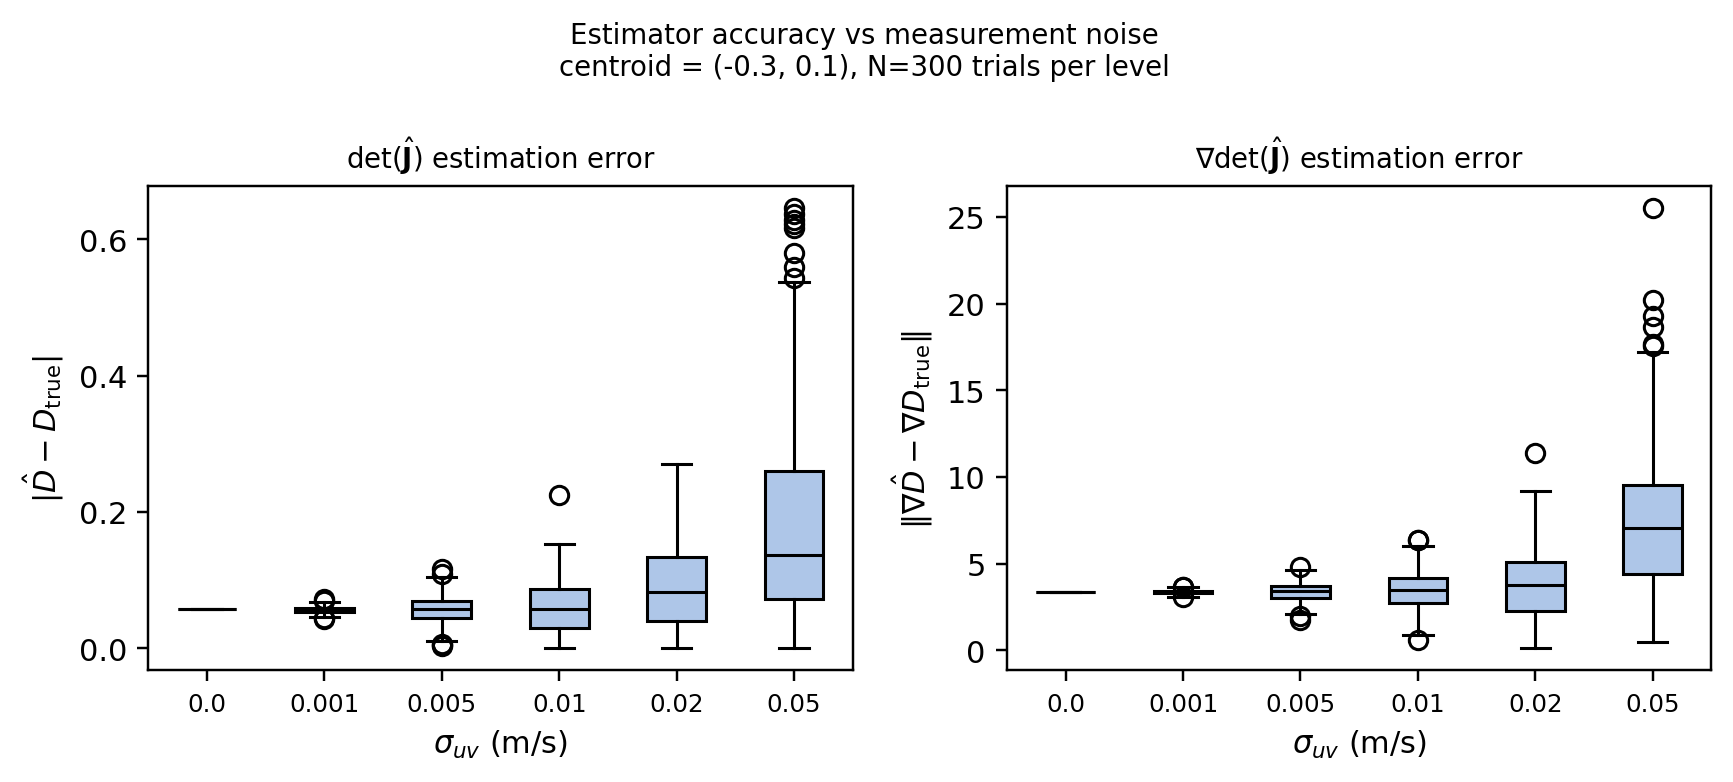
\includegraphics[width=0.45\textwidth]{figures/estimator_accuracy_vs_noise.png}
    % Generated by experiments/estimator_accuracy_sweep.py (CSV data) and
    % experiments/plot_estimator_accuracy.py (figure), under
    % trunk/Python_Simulations/Vector_Fields/VF_Robot/. Review copy in
    % experiments/outputs/estimator_accuracy/.
    \caption{Relative estimation error of $\hat{D}$, $\nabla\hat{D}$, and
    $\hat{\mathbf{H}}_D$ (median over $2 \times 10^5$ noise draws per point;
    shaded interquartile range in (a)) for the steady double gyre of
    Section~\ref{sec:dg_example}, formation held static at the
    strain-region point $\mathbf{p}_c = (-0.35, -0.20)$. (a) Versus measurement noise $\sigma_{uv}$ at the nominal
    formation radius $\rho = 0.075$; the dashed line marks error equal to
    signal magnitude. (b) Versus formation radius $\rho$ at $\sigma_{uv} =
    0.01$; dotted curves are the noise-free truncation floors. $\hat{D}$
    and $\nabla\hat{D}$ exhibit the radius trade-off of (\ref{eq:rho_star});
    $\hat{\mathbf{H}}_D$ is limited by the structural model bias of
    Section~\ref{sec:sensitivity}.}
    \label{fig:est_accuracy}
\end{figure}

Estimator accuracy was measured open loop: the formation was held static
at the strain-region point $\mathbf{p}_c = (-0.35, -0.20)$ of the steady
double gyre, $2 \times 10^5$ independent noise draws were applied per
condition through the same fit used by the controller, and the estimates
were compared with the analytic values of Appendix~\ref{app:analytic}.
The empirical standard deviation of every fitted coefficient matched the
closed forms of Lemma~\ref{lem:gains} within 0.2\%, and the per-robot
reading error induced by position noise matched the first-order
prediction of Section~\ref{sec:noise_model} within 1\%, confirming that
the two noise channels combine into a single effective measurement noise.

Fig.~\ref{fig:est_accuracy} reports the accuracy of the three navigation
quantities as relative error, the error magnitude divided by the
magnitude of the true quantity; a value of one (dashed line) means the
estimate is as wrong as it is large and carries no directional
information. In Fig.~\ref{fig:est_accuracy}(a) the three curves rise
linearly with $\sigma_{uv}$ and sit stacked a constant factor apart: each
additional derivative order multiplies the noise gain by roughly
$1/\rho$, about 13 at the nominal radius, the ladder of
Lemma~\ref{lem:gains}. Reading off the crossings of the dashed line,
$\hat{D}$ remains informative up to $\sigma_{uv} \approx 0.06$ m/s and
$\nabla\hat{D}$ up to $\sigma_{uv} \approx 0.01$ m/s, while
$\hat{\mathbf{H}}_D$ sits at the line even for the quietest sensors:
below $\sigma_{uv} \approx 0.005$ its error is set by the structural
model bias of Section~\ref{sec:sensitivity}, not by noise.
Fig.~\ref{fig:est_accuracy}(b) fixes $\sigma_{uv} = 0.01$ and varies the
formation radius. Enlarging the ring averages noise over a longer
baseline, so the solid curves fall; the quadratic model simultaneously
fits the curved field more poorly, so the noise-free truncation floors
(dotted) rise. The compromise of (\ref{eq:rho_star}) appears as minima
at $\rho \approx 0.11$ for $\hat{D}$ and $\rho \approx 0.23$ for
$\nabla\hat{D}$. These optima are properties of the double gyre at this
location and noise level, entering through the third-derivative scale
$M_3$; the one-third-power scaling law is general, but a different
field, or a different region of the same field, shifts them.
$\hat{\mathbf{H}}_D$ exhibits no minimum: its floor is radius
independent, as predicted, and no formation size improves it, though its
eigen-directions remain accurate to $0.35^\circ$ on and near the
separatrix and $3.8^\circ$ at the generic test point
(Remark~\ref{rem:eigvec}).

The gradient threshold locates where closed-loop degradation should
begin: at $\sigma_{uv} \approx 0.01$ a single $\nabla\hat{D}$ estimate
is as wrong as it is right, so any one control decision approaches
chance. The closed loop does not extend this limit: the Monte Carlo
sweep that follows places the tracker's 50\% success level at
$\sigma_{uv} \approx 0.01$, coinciding with the single-estimate
threshold. Saturation and the per-cycle redraw of the noise bound the
damage of individual bad commands, but they buy no additional margin
for a traverse that requires a long sequence of correct decisions.

\subsection{Simulation Results}

\begin{figure}[!t]
    \centering
    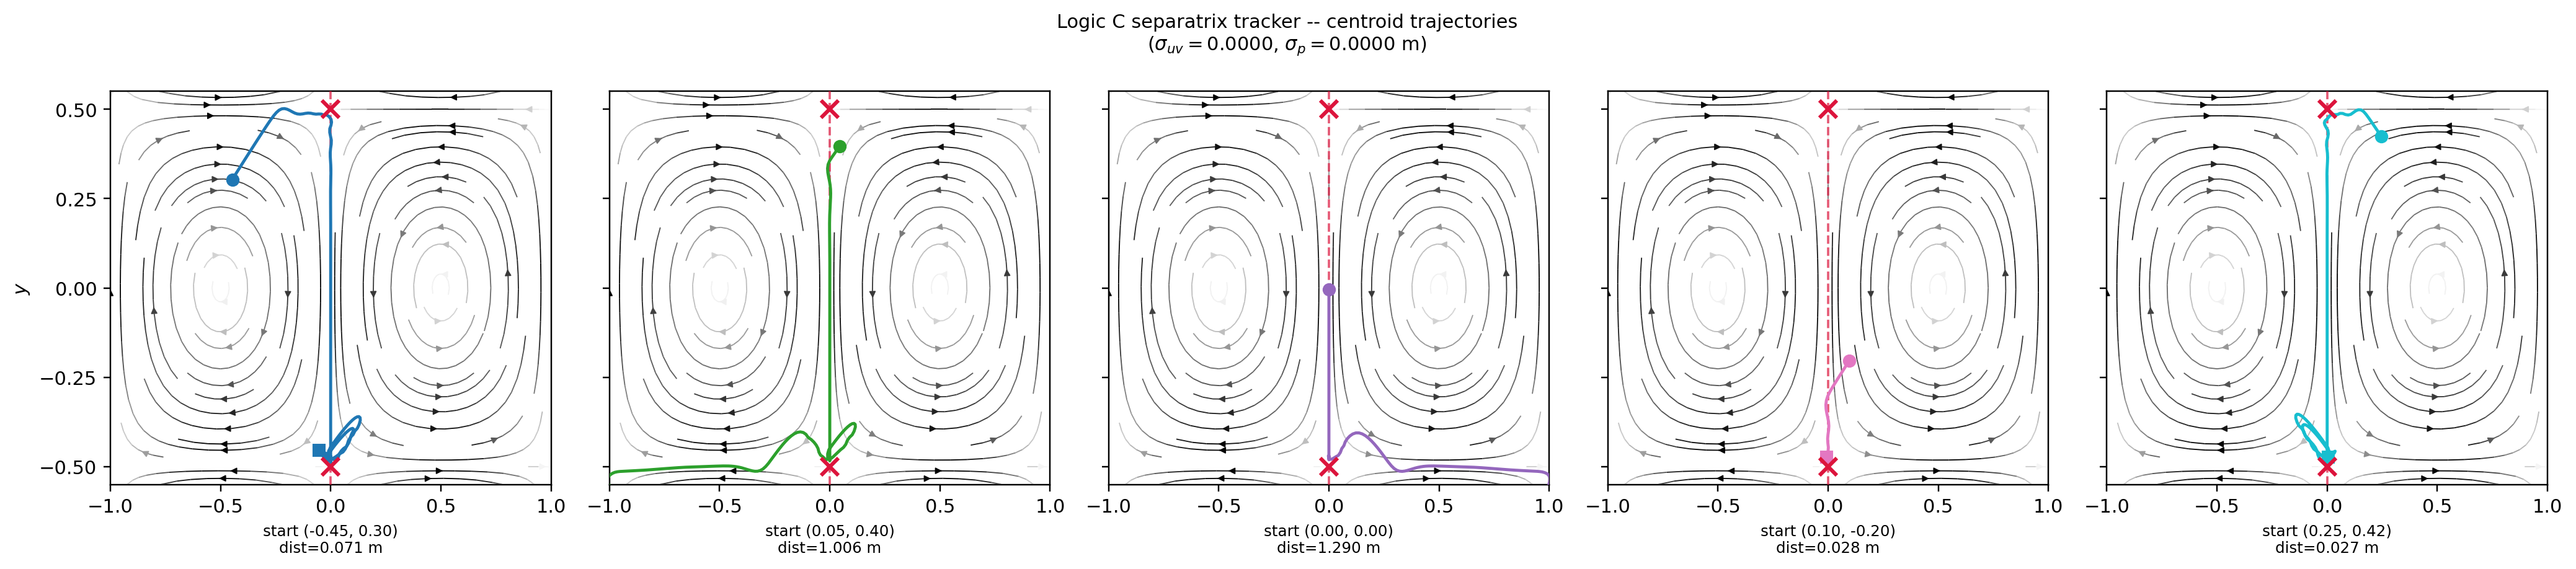
\includegraphics[width=0.45\textwidth]{figures/separatrix_trajectories.png}
    % Generated by experiments/separatrix_clean_runs.py, under
    % trunk/Python_Simulations/Vector_Fields/VF_Robot/. Review copy in
    % experiments/outputs/separatrix_clean/.
    \caption{Separatrix tracker (Logic C) centroid trajectories from six
    initial conditions, noise-free case, overlaid on the double-gyre
    streamlines and the two Okubo-Weiss diamonds. Start points are
    $\bullet$, saddles are $\times$. Every trajectory reaches $x = 0$ and
    continues along the wall trench through the terminal (bottom) saddle
    in both directions; a trial stops at domain exit or 150 steps after
    first saddle contact.}
    \label{fig:sep_trajectories}
\end{figure}

From the six starts of Fig.~\ref{fig:sep_trajectories}, all six reach the
separatrix and pass within 0.02 of the bottom saddle
$\mathbf{p}^*_1$ (closest approach 0.0003--0.0194 across runs). Three of
the six begin already inside the FLOW band and band immediately;
the other three take 6, 18, and 35 steps. Mode occupancy over each run
is FLOW 6--37\%, SLIDE 34--48\%, and ATTRACT 10--24\%, with the
remaining time split between the flow-drift and attract-fallback
refinements of the same three modes; no run spends more than a few
percent of its steps outside these categories. Every run continues past
the terminal saddle rather than stopping there. This traces to the
structural bias of $\hat{\mathbf{H}}_D$ (Section~\ref{sec:sensitivity}):
near the well the estimated eigenvalues are indefinite and roughly an
order of magnitude too small, so the capture test
$\lambda_1\lambda_2 \geq 0$ of Section~\ref{sec:sep_controller} does not
fire even without noise. Section~\ref{sec:discussion} returns to this
behavior, continuous traversal of the separatrix network, with terminal
capture demonstrated as a tightened-threshold special case.

\begin{table}[!t]
\centering
\caption{Separatrix tracker: success rate (traverse) by noise cell,
1000 trials/cell, fixed straddling start $(0, 0.35)$}
\label{tab:sep_success}
\footnotesize
\setlength{\tabcolsep}{4pt}
\begin{tabular}{r|rrrrr}
\hline
$\sigma_{uv}$ \textbackslash\ $\sigma_p$ & 0.000 & 0.005 & 0.010 & 0.020 & 0.050 \\
\hline
0.000 & 100.0 & 64.7 & 45.4 & 36.0 & 18.8 \\
0.001 &  99.3 & 61.9 & 43.7 & 33.8 & 19.9 \\
0.005 &  60.2 & 53.6 & 40.7 & 29.7 & 17.4 \\
0.010 &  43.3 & 40.6 & 39.6 & 28.1 & 18.4 \\
0.020 &  27.6 & 27.5 & 22.9 & 20.4 & 18.4 \\
0.050 &  15.1 & 16.4 & 14.7 & 15.2 & 15.0 \\
0.100 &  13.0 & 15.0 & 13.3 & 14.3 & 13.5 \\
\hline
\end{tabular}
\end{table}

Table~\ref{tab:sep_success} reports traverse success (reaching the
terminal saddle without formation collapse) over the noise grid. At
$\sigma_p = 0$ the rate is a clean step: 100\% through
$\sigma_{uv} = 0.001$, then falling through the 50\% level between
$\sigma_{uv} = 0.005$ and $0.01$, landing at 43.3\% at
$\sigma_{uv} = 0.01$. This coincides with the open-loop
$\nabla\hat{D}$ reliability threshold reported above
($\sigma_{uv} \approx 0.01$, ratio 1.0): saturation and per-cycle
resampling do not extend the noise budget
of a long decision sequence beyond what a single gradient estimate can
support. Position noise degrades the rate along the same curve scaled
by $\|\mathbf{J}\|$, consistent with the effective-noise argument of
Section~\ref{sec:noise_model}: $\sigma_p = 0.01$ alone gives 45.4\%,
close to $\sigma_{uv} = 0.01$ alone at 43.3\%. Beyond the cliff, success
does not fall to zero but levels off near 13--15\%: at this noise level
the controller behaves as an unbiased random walk that occasionally
lands on the saddle by chance, so the straddle-retention metric of
Table~\ref{tab:sep_straddle} is the sharper failure indicator. Tracking
error over the on-trench phase (mean $|x_c|$) rises from 0.002 m at zero
noise to 0.086 m at the $\sigma_{uv} = 0.01$ cliff and saturates near
0.27 m at high noise (comparable to the domain half-width), reflecting
trials that never band at all. Success was independent of initial
heading to within the sampling noise of the sweep (quartile success
74.9--76.2\% at low noise, confirming the isotropy of
Lemma~\ref{lem:gains}).

\begin{table}[!t]
\centering
\caption{Separatrix tracker: straddle retention by noise cell (fraction
of 1000 trials, Michini-comparable metric \cite{9})}
\label{tab:sep_straddle}
\footnotesize
\setlength{\tabcolsep}{4pt}
\begin{tabular}{r|rrrrr}
\hline
$\sigma_{uv}$ \textbackslash\ $\sigma_p$ & 0.000 & 0.005 & 0.010 & 0.020 & 0.050 \\
\hline
0.000 & 1.000 & 0.625 & 0.417 & 0.338 & 0.164 \\
0.005 & 0.560 & 0.493 & 0.365 & 0.272 & 0.157 \\
0.010 & 0.379 & 0.366 & 0.361 & 0.258 & 0.165 \\
0.020 & 0.237 & 0.232 & 0.187 & 0.177 & 0.159 \\
0.050 & 0.126 & 0.137 & 0.112 & 0.128 & 0.122 \\
\hline
\end{tabular}
\end{table}

\subsection{Ocean HFR Simulation}
\label{sec:results_ocean}

The separatrix tracker was run on the real, time-varying current field
of Section~\ref{sec:ocean_sim} from a single start north of the Santa
Barbara Channel entrance, $(34.40^{\circ}\mathrm{N},
-120.39^{\circ}\mathrm{W})$, using the operating point of
Table~\ref{tab:ocean_params}. Fig.~\ref{fig:ocean_progression} shows the
path building up over the full 28-h trial against the instantaneous
current field at five points in time: the cluster descends through the
channel entrance, tracks the ridge through the bifurcation near
$(34.1^{\circ}\mathrm{N}, -120.4^{\circ}\mathrm{W})$, and continues to
landfall on the middle island's north coast. Fig.~\ref{fig:ocean_ftle}
places the same trial against the 24-h forward-time FTLE field, computed
offline over the same window in the style of \cite{17}; the cluster's path
follows the dominant FTLE ridge running from the channel entrance to the
bifurcation closely, without the ridge being available to the controller
at any point, only the local $\hat{D}$ and $\hat{\mathbf{g}}$ estimates
that Section~\ref{sec:estimation} builds from the current samples at the
formation.

\begin{figure}[!t]
    \centering
    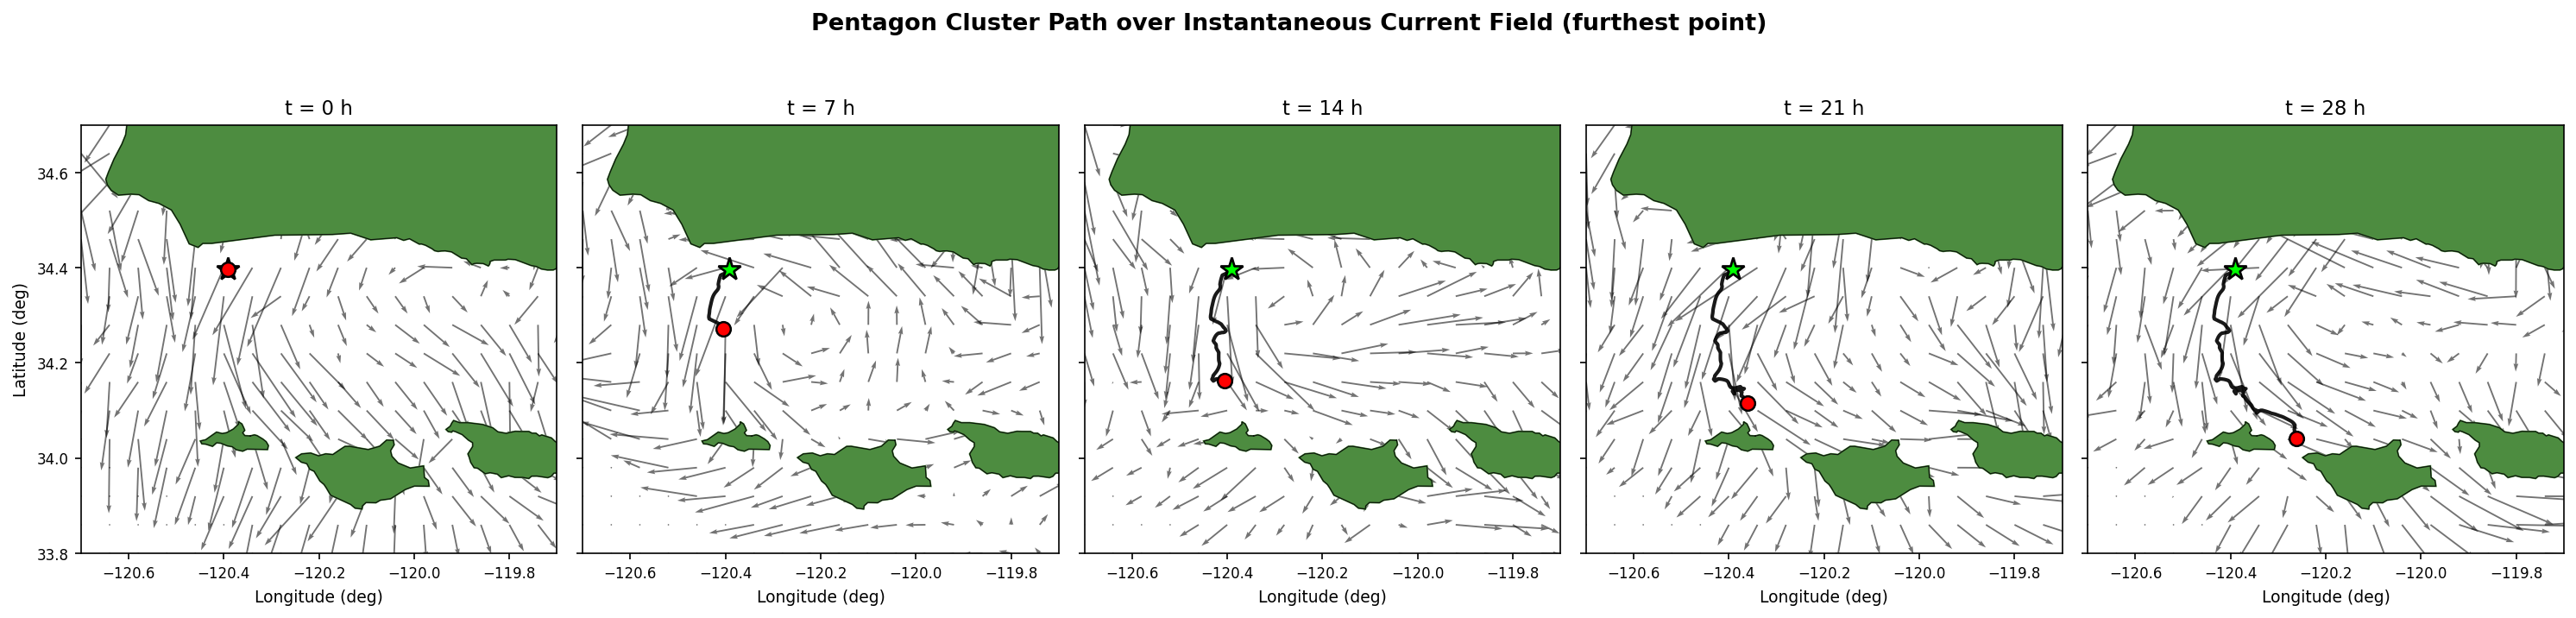
\includegraphics[width=0.48\textwidth]{figures/ocean_panel_progression_2km.png}
    % Generated by experiments/ocean_hfr_2km_panel_progression.py, under
    % trunk/Python_Simulations/Vector_Fields/VF_Robot/. Full-resolution
    % copy in ocean_data/det_jacobian_plots/ocean_panel_progression_2km.png.
    \caption{Centroid path so far (black) over the instantaneous current
    field (quiver), at $t = 0, 7, 14, 21, 28$~h into the 28-h trial. Green
    star is the start; red circle is the current position at each panel's
    time. The cluster descends through the channel entrance and turns
    toward the middle island as the current field evolves.}
    \label{fig:ocean_progression}
\end{figure}

\begin{figure}[!t]
    \centering
    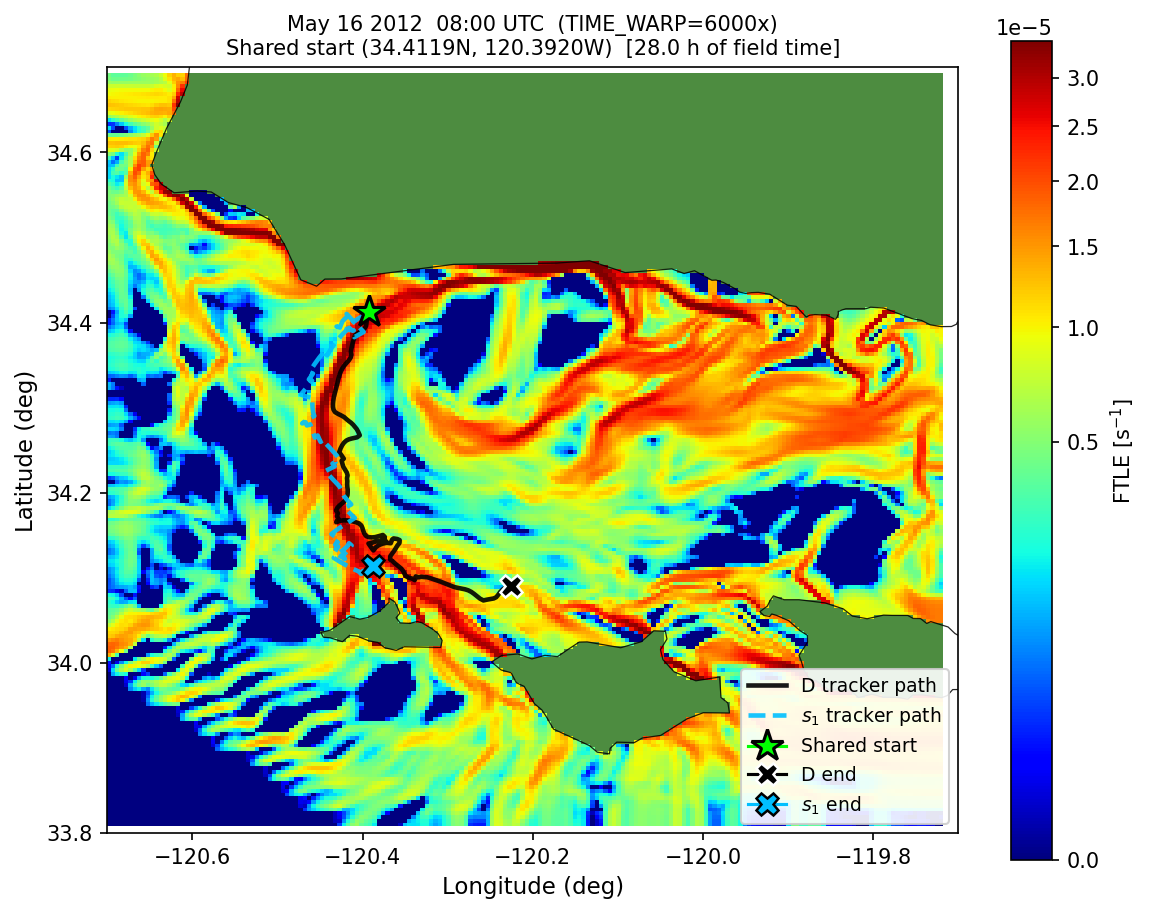
\includegraphics[width=0.48\textwidth]{figures/ocean_ftle_trajectory_overlay_2km.png}
    % Generated by experiments/main_ocean_hfr_2km_ftle_overlay.py, under
    % trunk/Python_Simulations/Vector_Fields/VF_Robot/. Full-resolution
    % copy in ocean_data/det_jacobian_plots/ftle_trajectory_overlay_2km.png.
    \caption{Full 28-h centroid and robot paths overlaid on the 24-h
    forward-time FTLE field computed from the same 2~km data. The path
    tracks the dominant ridge from the channel entrance to the
    bifurcation and continues to landfall near
    $(34.04^{\circ}\mathrm{N}, -120.26^{\circ}\mathrm{W})$.}
    \label{fig:ocean_ftle}
\end{figure}

Fig.~\ref{fig:ocean_ftle_snapshots} computes the same 24-h-style
forward FTLE anew at four anchor times spread through the record
(0, 5, 10, and 16~h, each integrated 12~h forward, the longest common
window the 29-frame archive supports at more than two anchors), showing
that the dominant ridge through the channel entrance persists across
the record while its finer structure downstream continues to evolve.
This is the sense in which the ocean experiment is genuinely
time-varying, unlike the steady double gyre of the rest of the paper:
the structure the controller tracks is not fixed in advance and the
controller has no access to its future evolution, only the
instantaneous samples at the current formation position.

\begin{figure*}[!t]
    \centering
    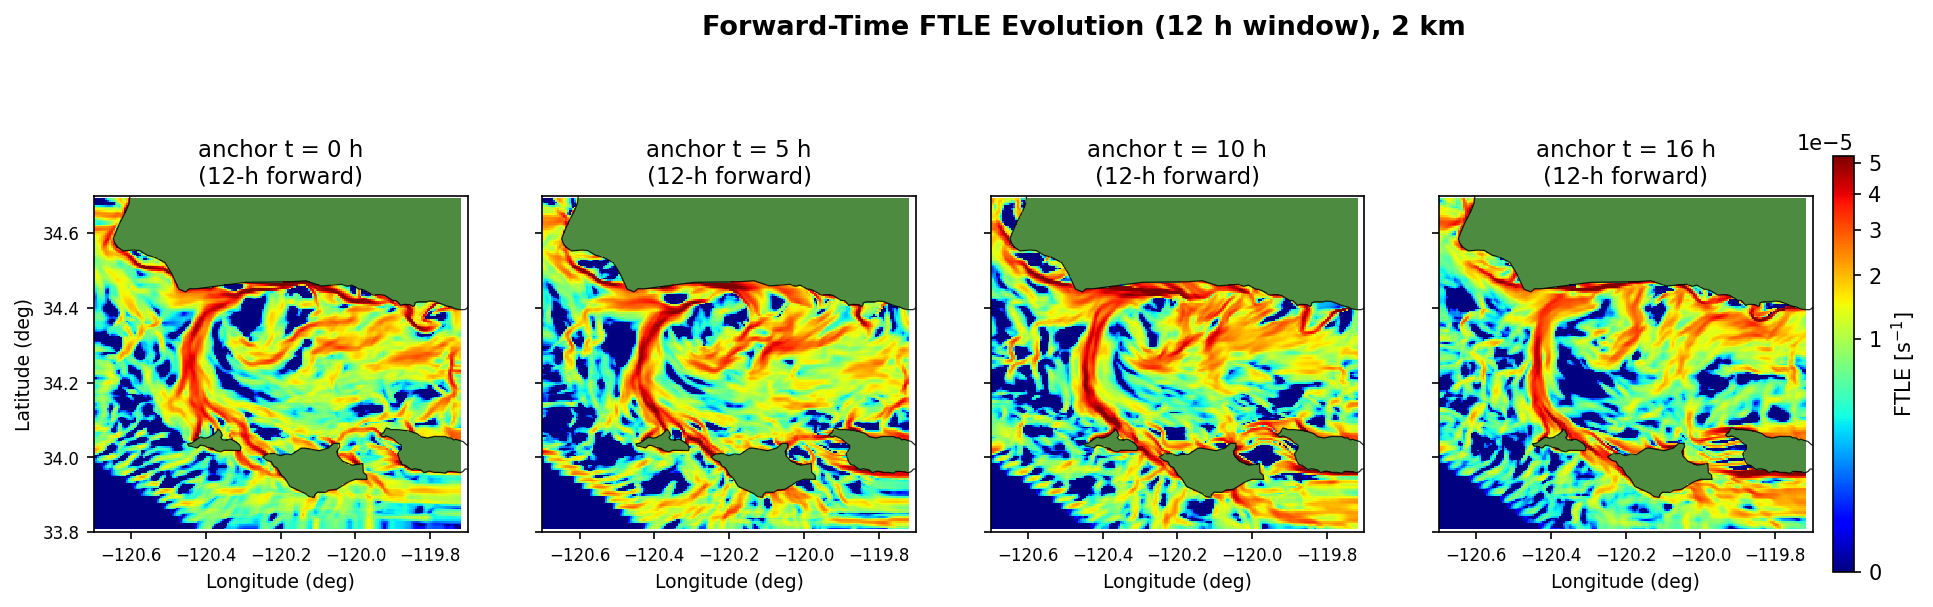
\includegraphics[width=0.9\textwidth]{figures/ocean_ftle_snapshots_2km.png}
    % Generated by experiments/ocean_hfr_2km_ftle_snapshots.py, under
    % trunk/Python_Simulations/Vector_Fields/VF_Robot/.
    \caption{Forward-time FTLE (12-h window) anchored at four times
    across the 28-h record. The dominant ridge through the channel
    entrance is stable across all four anchors; downstream structure
    continues to evolve, confirming the field is genuinely time-varying
    over the trial.}
    \label{fig:ocean_ftle_snapshots}
\end{figure*}

Fig.~\ref{fig:ocean_branch} tests the trial's sensitivity to the start
position with a $10 \times 10$ grid of starts jittered
$\pm 0.05^{\circ}$ around the validated start, each run through the
full 28-h trial. Of the 100 starts, 84 land on the same
middle-island branch as the validated trial; the remaining 16, all at
the edges of the jitter box furthest from the ridge, are carried onto a
western branch that does not make landfall in the domain. The mean
distance from a start to the 95th-percentile FTLE ridge contour was
1.4~km, small relative to the $\sim 0.3^{\circ}$ ($\sim 33$~km) domain
radius, so the branch boundary sits close to the jitter box: most of
the box is on one side of it. This is a basin-of-attraction result in
the sense of Section~\ref{sec:limitations}, not a robustness guarantee;
it shows that the tracked branch is the typical outcome for starts near
the validated one, not that every start converges to it.

\begin{figure}[!t]
    \centering
    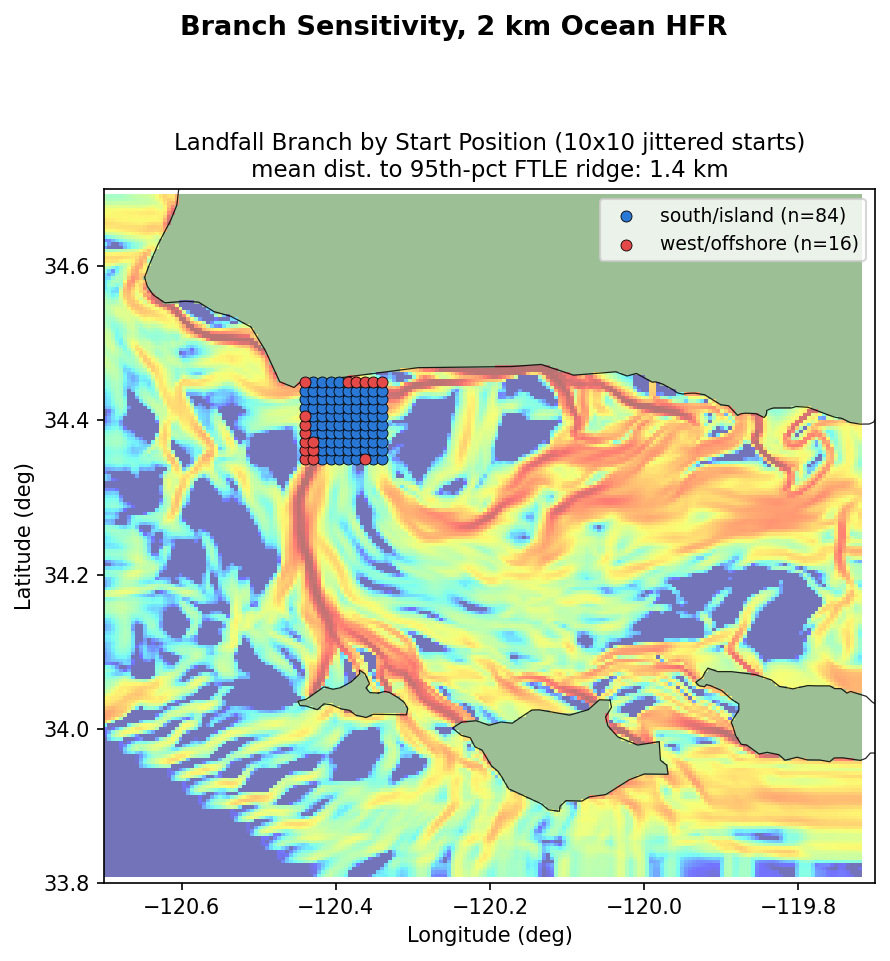
\includegraphics[width=0.48\textwidth]{figures/ocean_branch_sensitivity_2km.png}
    % Generated by experiments/ocean_hfr_2km_branch_sensitivity.py, under
    % trunk/Python_Simulations/Vector_Fields/VF_Robot/. Per-trial data in
    % ocean_data/det_jacobian_plots/ocean_branch_sensitivity_2km.csv.
    \caption{Landfall branch for a $10 \times 10$ grid of starts jittered
    around the validated start, over the 24-h forward FTLE background.
    84 of 100 starts (blue) reach the same middle-island branch as
    Fig.~\ref{fig:ocean_ftle}; 16 (red), all near the jitter box edges,
    are carried onto a western branch instead.}
    \label{fig:ocean_branch}
\end{figure}


% ---------------------------------------------------------------------------
\section{Discussion}
\label{sec:discussion}

\subsection{Implications for Distributed Eulerian-Structure Following}

The stability result of Section~\ref{sec:stability} is harder to obtain
than a codimension-one regular-level-set tracking result would be,
for a structural reason. A regular level set of a scalar field is
determined by first-order information alone: a gradient that does not
vanish fully fixes the transversal direction, and a controller built
from it admits a global certificate from a single quadratic Lyapunov
function. The separatrix trench lives where that first-order
information vanishes in the normal direction, so any controller and any
proof must synthesize the missing direction from curvature; the
eigenstructure dependence, mode switching, and tube assumptions of
Section~\ref{sec:stab_sep} are the price of that synthesis.

The results of Section~\ref{sec:results} show that a six-robot formation
sampling only its own local velocities recovers enough second-order
structure, not the field itself, to find and follow this Eulerian
feature, with no map, no forecast, and no communication beyond the
single synchronous sample each control cycle already requires. The
$\det(\mathbf{J})$ landscape is what makes this possible: the separatrix
reduces to following a scalar surrogate field, the trench, computable
from the same twelve fitted coefficients that recover the Jacobian,
rather than to any procedure specific to streamlines or Lagrangian
integration. The trench is a curve defined by where curvature
information vanishes to first order and must instead be supplied by
the Hessian, which is precisely why this problem needs the Hessian
estimator of Section~\ref{sec:estimation} rather than the gradient
estimate a first-order feature would require.

\subsection{Park versus Traverse: One Threshold, Two Behaviors}
\label{sec:park_vs_traverse}

Theorem~\ref{thm:separatrix} and Remark~\ref{rem:capture_gap} identify
the terminal-capture test $\lambda_1\lambda_2 \geq 0$ as the reason the
deployed controller continues through every saddle in
Section~\ref{sec:results}: the biased $\hat{\mathbf{H}}_D$ makes that
test unreliable exactly where it would need to fire. An estimator-aware
alternative restores capture without touching the transverse Newton
snap, the flow step, or the slide step, using only the two quantities
Section~\ref{sec:sensitivity} shows are linear in the fitted
coefficients and free of the Hessian's structural bias, $\hat{D}$ and
$\hat{\mathbf{g}}$. The \emph{park step} adds a fourth mode, checked
before the FLOW test:
\begin{equation}
    \text{if } \hat{D} < D_{\text{capture}}:\quad
    \dot{\mathbf{p}}_c^{\,\text{des}} =
    -\begin{bmatrix}
        \mathrm{sat}(\hat{g}_x) \\ \mathrm{sat}(\hat{g}_y)
    \end{bmatrix},
    \label{eq:park_step}
\end{equation}
componentwise saturated gradient descent on $\hat{D}$, which converges
to the nearest local minimum of $D$, the flow saddle at the end of the
current trench segment, exactly as Theorem~\ref{thm:attract} predicts
for the exact-estimate case. $D_{\text{capture}}$ is the one-parameter
knob: $D_{\text{capture}} = -\infty$ disables the test and the
controller is trajectory-identical to Logic C (verified in
\textit{separatrix\_logic\_park\_step}, bit-exact off), while a finite
threshold inside the well (here $-0.5$, roughly half the double-gyre
well depth $\pi^4 A^2 \approx 0.974$) parks the team there.
Fig.~\ref{fig:park_vs_traverse} runs both settings from the same start,
noise-free: traverse exits the domain at $(1.00, -0.51)$ after 228
steps, riding the crossing trench as Section~\ref{sec:results}
describes; park reaches the saddle and holds position with zero
tail-position standard deviation over its final 100 steps, settling
0.0124~m from $\mathbf{p}^*_1$. Both runs use the identical estimation
step and the identical selector below the park test; the only
difference is one threshold. This is the practical resolution of
Remark~\ref{rem:capture_gap}: continuation is not a controller limitation
to be designed around so much as the honest behavior of the theorem's
capture test under a real estimator, and a single threshold recovers
whichever behavior a mission calls for, terminal parking at a critical
point or open-ended traversal of the network.

\begin{figure}[!t]
    \centering
    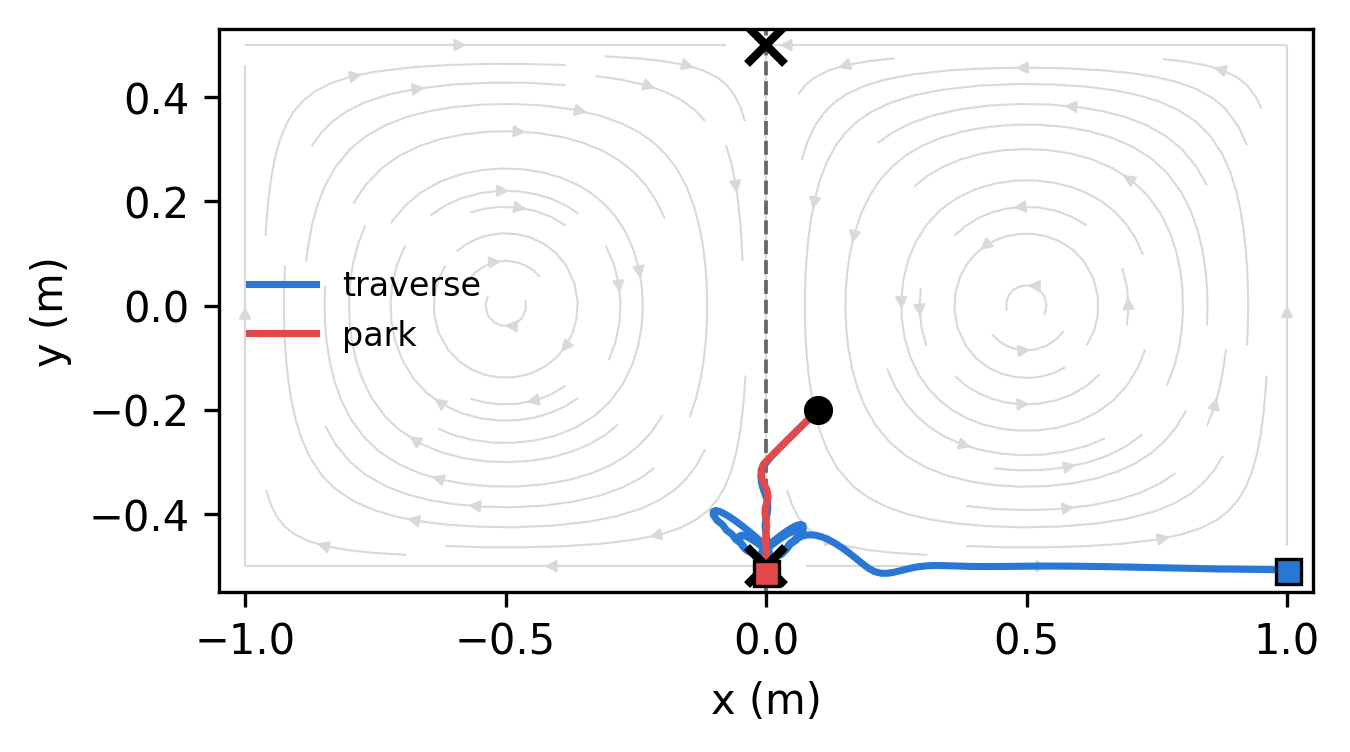
\includegraphics[width=0.45\textwidth]{figures/park_vs_traverse.png}
    % Generated by experiments/park_vs_traverse_demo.py, under
    % trunk/Python_Simulations/Vector_Fields/VF_Robot/. Review copy in
    % experiments/outputs/separatrix_clean/.
    \caption{Park versus traverse from the same start $(0.10, -0.20)$,
    noise-free. Traverse (Logic C) rides the trench through the bottom
    saddle and exits the domain. Park (Logic Park,
    $D_{\text{capture}} = -0.5$) applies the park step
    (\ref{eq:park_step}) once $\hat{D}$ drops below threshold and holds
    the team 0.0124~m from the saddle.}
    \label{fig:park_vs_traverse}
\end{figure}

\subsection{Failure Modes}

Two behaviors fall outside the guarantees of
Section~\ref{sec:stability} and are worth stating plainly rather than
leaving implicit. First, the estimator is ill-conditioned whenever the
six sampling points drift toward a common conic
(Proposition~\ref{prop:conic}): $\det(\boldsymbol{\Phi})$ shrinks
continuously as the formation deforms toward one, and the fitted
coefficients degrade smoothly until, at the conic itself, the fit is
undefined. A ring formation without a center robot is the standing
example (Remark following Corollary~\ref{cor:pentagon}); the pentagon
plus center used throughout is one robot away from this failure by
construction, but a controller could in principle drive the formation
toward a degenerate shape through rotation or scaling commands not
considered here. Monitoring $\det(\boldsymbol{\Phi})$, or equivalently
the interior angles of the formation, and adding a shape-maintenance
term to the centroid command is the direct mitigation; the Monte Carlo
trials of Section~\ref{sec:results} flag the weaker symptom, an
inter-robot distance excursion beyond twice the nominal pair length, as
a formation collapse, and it does not occur in any reported trial.

Second, the separatrix controller can chatter across the FLOW-band
boundary (\ref{eq:flow_band}) when the centroid sits near the threshold
and noise pushes $\hat{D}$ or the dimensionless ratio
$|\hat{D}|/\|\hat{\mathbf{H}}_D\|_F$ back and forth across
$\varepsilon_{\text{dim}}$. Because every mode shares the transverse
dynamics (\ref{eq:n_dynamics}), chatter does not destabilize the
transverse channel; its cost is tangential, a lower effective
along-trench speed as the command alternates between the flow step and
the slide or attract step. $\varepsilon_{\text{dim}}$ trades this
against the crest crossing of Section~\ref{sec:dg_example}: too small a
threshold reintroduces the stall the flow-assisted mode was built to
remove, too large a threshold widens the band and the chatter with it.
The value used throughout, $\varepsilon_{\text{dim}} = 0.025$, was fixed
once and not retuned per experiment.


% ---------------------------------------------------------------------------
\section{Limitations}
\label{sec:limitations}

This paper restricts attention to the static double gyre ($\varepsilon = 0$).
In the time-varying case ($\varepsilon > 0$) the separatrix becomes a
material curve that evolves with the flow; tracking it would require
adapting the control law to account for the flow unsteadiness. This
extension is left to future work.

Results are presented for a single field family (the double gyre). Whether
the separatrix tracker generalizes to other fields with saddle-like
regions is not addressed here, though the estimation framework
(Section~\ref{sec:estimation}) applies to any smooth planar vector field.

All results are from simulation only. Hardware validation on the Decabot
testbed is not reported in this paper; it is planned as a follow-on study.

The stability guarantees, and the reported success rates, are local.
Theorem~\ref{thm:separatrix} assumes initialization inside the tube
$T_w$, and all Monte Carlo trials start from a formation straddling the
separatrix. The attract mode converges to the critical set of $D$, which
includes the gyre-center maxima, so a team started deep inside a vortex
core parks at the core rather than on the separatrix: in supplementary
uniform-random-start trials over the domain, roughly half (47.9\%,
$n = 1000$) of starts reached the trench at zero noise. We do not
characterize the basin of attraction of the separatrix; prior
adaptive-navigation primitives \cite{27}, \cite{28} likewise report local
convergence without basin estimates.


% ---------------------------------------------------------------------------
\section{Future Work}
\label{sec:future}

Direct extensions of this work include:
\begin{itemize}
    \item \textbf{Time-varying double gyre.} The ocean HFR experiment of
          Section~\ref{sec:results_ocean} shows the controller already
          operates on a genuinely time-varying field without modification;
          a time-derivative correction term to the navigation primitive,
          analyzed against the analytic $\varepsilon > 0$ double gyre where
          the exact structure motion is known, would let the stability
          results of Section~\ref{sec:stability} extend to that case with
          a quantified bound rather than empirical evidence alone.
    \item \textbf{Online formation reshaping.} Adapting the pair lengths
          $(L_k)$ and the SAS parameters to improve the conditioning of
          $\boldsymbol{\Phi}$ when the cluster is near a degenerate
          configuration.
    \item \textbf{Hardware deployment.} Validating the controller on the
          Decabot testbed using the OptiTrack motion-capture system. The
          separatrix can be represented by a vector field emitted by an
          on-board computer and sampled by the robots' onboard sensors.
    \item \textbf{Extension to 3D.} Generalizing the quadratic estimator
          to three-dimensional fields, which would require at least 10 robots
          per component for full cubic determination, or a reduced-order
          estimator with different assumptions.
\end{itemize}


% ---------------------------------------------------------------------------
\section{Conclusion}
\label{sec:conclusion}

This paper presented a distributed framework for navigating a six-robot
formation along the separatrix of the double gyre. A quadratic
estimator using simultaneous measurements from the six robots recovers the
Jacobian, its determinant $D = \det(\mathbf{J})$, gradient, and Hessian at
the cluster centroid with no prior field knowledge, with closed-form noise
gains verified empirically to within $0.2\%$. An adaptive controller built
on a modified Newton step was derived, with a Lyapunov stability
certificate that additionally extends to a network-traversal theorem,
since the trench of $D$ a controller reaches continues through every
saddle it crosses rather than terminating there, with single-saddle
capture recovered as a tightened-threshold special case demonstrated in
simulation. Monte Carlo simulation over a two-dimensional noise sweep
placed the tracker's 50\% success level at $\sigma_{uv} \approx 0.01$,
exactly the level at which a single gradient estimate stops being
informative: the estimator, not the control law, sets the noise ceiling.
On real, time-varying current data from the Santa Barbara Channel the
separatrix tracker followed the dominant coherent-structure ridge for
28 hours of field time to a consistent landfall, reproduced by 84 of
100 nearby starts, using only the same local estimates validated in
simulation, with no forecast, map, or access to the field's future
evolution.


\appendices

% ---------------------------------------------------------------------------
\section{Double-Gyre Analytic Forms}
\label{app:analytic}

For the steady double gyre with amplitude $A$, $x_f = x + 1$,
$y_f = y + 0.5$, define $s_x = \sin(\pi x_f)$, $c_x = \cos(\pi x_f)$,
$s_y = \sin(\pi y_f)$, $c_y = \cos(\pi y_f)$. The field is
$u = -\pi A s_x c_y$, $v = \pi A c_x s_y$.

The Jacobian entries are
\begin{equation}
    \frac{\partial u}{\partial x} = -\pi^2 A c_x c_y, \quad
    \frac{\partial u}{\partial y} =  \pi^2 A s_x s_y,
\end{equation}
\begin{equation}
    \frac{\partial v}{\partial x} = -\pi^2 A s_x s_y, \quad
    \frac{\partial v}{\partial y} =  \pi^2 A c_x c_y,
\end{equation}
so the flow is divergence free and
\begin{equation}
    \begin{split}
    D = \det(\mathbf{J})
      &= -\pi^4 A^2 \bigl(c_x^2 c_y^2 - s_x^2 s_y^2\bigr) \\
      &= -\frac{\pi^4 A^2}{2}\bigl(\cos 2\pi x_f + \cos 2\pi y_f\bigr),
    \end{split}
    \label{eq:det_analytic}
\end{equation}
using $c^2 = (1+\cos 2\alpha)/2$ and $s^2 = (1-\cos 2\alpha)/2$. $D$ is
positive at the gyre centers ($D = \pi^4 A^2$), negative at the corner
saddles ($D = -\pi^4 A^2$), and zero on the diamonds
$x_f \pm y_f \in \tfrac{1}{2} + \mathbb{Z}$, by the factorization
$\cos 2\pi x_f + \cos 2\pi y_f = 2\cos\pi(x_f+y_f)\cos\pi(x_f-y_f)$.

Differentiating (\ref{eq:det_analytic}),
\begin{equation}
    \begin{aligned}
    \nabla D &= \pi^5 A^2
    \begin{bmatrix} \sin 2\pi x_f \\ \sin 2\pi y_f \end{bmatrix},
    \\
    \mathbf{H}_D &= 2\pi^6 A^2
    \begin{bmatrix} \cos 2\pi x_f & 0 \\ 0 & \cos 2\pi y_f \end{bmatrix}.
    \end{aligned}
    \label{eq:gradhess_analytic}
\end{equation}
The Hessian is diagonal everywhere, so $D$ is additively separable in
$x_f$ and $y_f$, which is what makes the trench normal form of
Assumption~\ref{ass:trench} exact for this field. The vorticity is
$\omega = -2\pi^2 A s_x s_y$, which vanishes on the separatrix
$x_f = 1$; there $\mathbf{J}$ is symmetric and $\sqrt{-D}$ is the
exact instantaneous strain rate. The Okubo-Weiss parameter is
$Q = -D$ by incompressibility, so the $Q = 0$ and $D = 0$ contours
coincide.


% ---------------------------------------------------------------------------
\section{Pentagon Cluster Kinematics}
\label{app:kinematics}

\subsection{Forward Kinematics}

The pentagon-of-pairs cluster has 6 robots indexed $i = 1, \ldots, 6$, arranged
as three pairs. Pair $k$ ($k = 1, 2, 3$) consists of robots $2k-1$ and $2k$.
The midpoint of pair $k$ is $\mathbf{m}_k = (\mathbf{p}_{2k-1} +
\mathbf{p}_{2k})/2$. The three midpoints form a triangle; the centroid of that
triangle is $\mathbf{p}_c = (\mathbf{m}_1 + \mathbf{m}_2 + \mathbf{m}_3)/3$.

The SAS parameters of the midpoint triangle are defined as in the three-robot
case: $p_1 = \|\mathbf{m}_2 - \mathbf{m}_1\|$, $q_1 = \|\mathbf{m}_3 -
\mathbf{m}_2\|$, and $\beta_1$ is the interior angle at $\mathbf{m}_2$.
The cluster heading $\theta_c = \text{atan2}(m_{2,y} - m_{1,y},
m_{2,x} - m_{1,x})$.

Each pair is described by its half-length $L_k/2$ and orientation angle
$\psi_k$, so the two robots in pair $k$ are at $\mathbf{m}_k \pm (L_k/2)
(\cos\psi_k, \sin\psi_k)^\top$.

The full 12-state cluster configuration is
$(x_c, y_c, \theta_c, p_1, \beta_1, q_1, L_2, \psi_2, L_3, \psi_3,
L_4, \psi_4)$, where pair 1 uses $L_1$ fixed and $\psi_1 = \theta_c$ by
convention.

\subsection{Inverse Kinematics}

Given the 12-state cluster configuration, the six robot positions are recovered
by:
\begin{enumerate}
    \item Constructing the midpoint triangle from $(p_1, \beta_1, q_1)$ in
          a local frame (following the same procedure as the three-robot
          cluster in Appendix B of \cite{14}).
    \item Rotating and translating to the global frame using $\theta_c$,
          $x_c$, $y_c$.
    \item Placing each pair of robots by offsetting from the midpoint along
          $(\cos\psi_k, \sin\psi_k)$ by $L_k/2$ in each direction.
\end{enumerate}

\subsection{Inverse Kinematic Jacobian}

The $12 \times 12$ inverse kinematic Jacobian maps desired cluster state
velocities $\dot{\boldsymbol{\xi}}$ to robot velocity commands
$(\dot{x}_1, \dot{y}_1, \ldots, \dot{x}_6, \dot{y}_6)^\top$:
\begin{equation}
    \begin{bmatrix} \dot{x}_1 \\ \dot{y}_1 \\ \vdots \\
    \dot{x}_6 \\ \dot{y}_6 \end{bmatrix}
    =
    \mathbf{J}_c^{-1}
    \begin{bmatrix} \dot{x}_c \\ \dot{y}_c \\ \dot{\theta}_c \\
    \dot{p}_1 \\ \dot{\beta}_1 \\ \dot{q}_1 \\
    \dot{L}_2 \\ \dot{\psi}_2 \\ \dot{L}_3 \\ \dot{\psi}_3 \\
    \dot{L}_4 \\ \dot{\psi}_4 \end{bmatrix},
    \label{eq:inv_kin_jac}
\end{equation}
where $\mathbf{J}_c^{-1}$ is a $12 \times 12$ matrix of partial derivatives
$\partial (x_i, y_i) / \partial \xi_j$ computed analytically from the inverse
kinematics. The explicit entries are omitted here for brevity; the
implementation is in \textit{pentagon\_kinematics.py}.


% ---------------------------------------------------------------------------
\begin{thebibliography}{99}

\bibitem{1} J. Cortés and M. Egerstedt, "Coordinated control of multi-robot
systems: A survey," \textit{SICE Journal of Control, Measurement, and
System Integration}, vol. 10, no. 6, pp. 495--503, 2017.

\bibitem{2} J. Das et al., "Coordinated sampling of dynamic oceanographic
features with underwater vehicles and drifters," \textit{The International
Journal of Robotics Research}, vol. 31, no. 5, pp. 626--646, 2012.

\bibitem{3} S. McCammon et al., "Ocean front detection and tracking using a
team of heterogeneous marine vehicles," \textit{Journal of Field Robotics},
vol. 38, no. 6, pp. 854--881, 2021.

\bibitem{4} S. R. Ramp et al., "Preparing to predict: the second autonomous
ocean sampling network (AOSN-II) experiment in the Monterey Bay,"
\textit{Deep Sea Research Part II: Topical Studies in Oceanography}, vol. 56,
no. 3-5, pp. 68--86, 2009.

\bibitem{5} C. Dong et al., "Oceanic mesoscale eddies," \textit{Ocean-Land-
Atmosphere Research}, vol. 4, p. 0081, 2025.

\bibitem{6} G. Haller and G. Yuan, "Lagrangian coherent structures and mixing
in two-dimensional turbulence," \textit{Physica D: Nonlinear Phenomena},
vol. 147, no. 3-4, pp. 352--370, 2000.

\bibitem{7} T. Peacock and G. Haller, "Lagrangian coherent structures: The
hidden skeleton of fluid flows," \textit{Physics Today}, vol. 66, no. 2,
pp. 41--47, 2013.

\bibitem{8} S. C. Shadden, F. Lekien, and J. E. Marsden, "Definition and
properties of Lagrangian coherent structures from finite-time Lyapunov
exponents in two-dimensional aperiodic flows," \textit{Physica D}, vol. 212,
no. 3-4, pp. 271--304, 2005.

\bibitem{9} M. Michini, M. A. Hsieh, E. Forgoston, and I. B. Schwartz,
"Robotic tracking of coherent structures in flows," \textit{IEEE Transactions
on Robotics}, vol. 30, no. 3, pp. 593--603, 2014.

\bibitem{10} M. Michini, H. Rastgoftar, M. A. Hsieh, and S. Jayasuriya,
"Distributed formation control for collaborative tracking of manifolds in
flows," in \textit{Proc. American Control Conference}, pp. 3874--3880, 2014.

\bibitem{11} M. Michini, M. A. Hsieh, E. Forgoston, and I. B. Schwartz,
"Experimental validation of robotic manifold tracking in gyre-like flows,"
in \textit{Proc. IEEE/RSJ International Conference on Intelligent Robots
and Systems (IROS)}, pp. 2306--2311, 2014.

\bibitem{12} G. Knizhnik, P. Li, X. Yu, and M. A. Hsieh, "Flow-based control
of marine robots in gyre-like environments," in \textit{Proc. 2022 Int. Conf.
on Robotics and Automation (ICRA)}, pp. 3047--3053, 2022.

\bibitem{13} D. Kularatne and M. A. Hsieh, "Tracking attracting manifolds in
flows," \textit{Autonomous Robots}, vol. 41, no. 8, pp. 1575--1588, 2017.

\bibitem{14} C. Waight and C. A. Kitts, "Adaptive navigation of multirobot
systems to critical points in 2D vector fields," \textit{IEEE/ASME Transactions
on Mechatronics}, to appear.

\bibitem{15} L. Briñón-Arranz, A. Renzaglia, and L. Schenato, "Multirobot
symmetric formations for gradient and Hessian estimation with application to
source seeking," \textit{IEEE Transactions on Robotics}, vol. 35, no. 3,
pp. 782--789, 2019.

\bibitem{16} G. Haller, "Lagrangian coherent structures," \textit{Annual
Review of Fluid Mechanics}, vol. 47, pp. 137--162, 2015.

\bibitem{17} M. Serra and G. Haller, "Objective Eulerian coherent
structures," \textit{Chaos: An Interdisciplinary Journal of Nonlinear
Science}, vol. 26, no. 5, p. 053110, 2016.

\bibitem{18} P. J. Nolan, M. Serra, and S. D. Ross, "Finite-time Lyapunov
exponents in the instantaneous limit and material transport,"
\textit{Nonlinear Dynamics}, vol. 100, no. 4, pp. 3825--3852, 2020.

\bibitem{19} T. D. Harms, S. T. M. Dawson, and B. J. McKeon, "Lagrangian
gradient regression for the detection of coherent structures from sparse
trajectory data," \textit{Royal Society Open Science}, vol. 11, no. 9,
p. 240586, 2024.

\bibitem{20} G. Haller, "Dynamic rotation and stretch tensors from a
dynamic polar decomposition," \textit{Journal of the Mechanics and Physics
of Solids}, vol. 86, pp. 70--93, 2016.

\bibitem{21} A. Okubo, "Horizontal dispersion of floatable particles in the
vicinity of velocity singularities such as convergences," \textit{Deep-Sea
Research}, vol. 17, no. 3, pp. 445--454, 1970.

\bibitem{22} J. Weiss, "The dynamics of enstrophy transfer in two-dimensional
hydrodynamics," \textit{Physica D: Nonlinear Phenomena}, vol. 48, no. 2-3,
pp. 273--294, 1991.

\bibitem{23} J. C. R. Hunt, A. A. Wray, and P. Moin, "Eddies, streams, and
convergence zones in turbulent flows," in \textit{Proc. Summer Program,
Center for Turbulence Research}, Rep. CTR-S88, pp. 193--208, 1988.

\bibitem{24} B.-L. Hua and P. Klein, "An exact criterion for the stirring
properties of nearly two-dimensional turbulence," \textit{Physica D}, vol. 113,
no. 1, pp. 98--110, 1998.

\bibitem{25} R. Cooper et al., "Initial study of multirobot adaptive
navigation for exploring environmental vector fields," in \textit{Proc.
IEEE Aerospace Conference}, 2019.

\bibitem{26} P. Ögren, E. Fiorelli, and N. E. Leonard, "Cooperative control
of mobile sensor networks: Adaptive gradient climbing in a distributed
environment," \textit{IEEE Transactions on Automatic Control}, vol. 49, no. 8,
pp. 1292--1302, 2004.

\bibitem{27} R. T. McDonald, C. A. Kitts, and M. A. Neumann, "Navigation of
scalar fronts with multirobot clusters in simulation and experiment,"
\textit{IEEE Systems Journal}, vol. 14, no. 3, pp. 3755--3766, 2020.

\bibitem{28} C. A. Kitts, R. T. McDonald, and M. A. Neumann, "Adaptive
navigation control primitives for multirobot clusters: Extrema finding,
contour following, ridge/trench following, and saddle point station keeping,"
\textit{IEEE Access}, vol. 6, pp. 17625--17642, 2018.

\bibitem{29} R. T. McDonald, C. A. Kitts, and M. A. Neumann, "Experimental
implementation and verification of scalar field ridge, trench, and saddle
point maneuvers using multirobot adaptive navigation," \textit{IEEE Access},
vol. 7, pp. 62950--62961, 2019.

\bibitem{30} C. A. Kitts and I. Mas, "Cluster space specification and control
of mobile multirobot systems," \textit{IEEE/ASME Transactions on Mechatronics},
vol. 14, no. 2, pp. 207--218, 2009.

\bibitem{31} T. Adamek, C. A. Kitts, and I. Mas, "Gradient-based cluster space
navigation for autonomous surface vessels," \textit{IEEE/ASME Transactions on
Mechatronics}, vol. 20, no. 2, pp. 506--518, 2014.

\bibitem{32} S. Tomer et al., "A low-cost indoor testbed for multirobot
adaptive navigation research," in \textit{Proc. IEEE Aerospace Conference},
pp. 1--12, 2018.

\bibitem{33} C. Waight and C. Kitts, "A functional indoor testbed for
multirobot adaptive navigation in vector field environments," in
\textit{Proc. ASME Int. Design Engineering Technical Conf. and Computers
and Information in Engineering Conf.}, vol. 89251, 2025.

\bibitem{34} Y. Sun, G. Ma, M. Liu, C. Li, and J. Liang, "Distributed
finite-time coordinated control for multi-robot systems with disturbances
and directed topologies," \textit{Transactions of the Institute of
Measurement and Control}, vol. 39, no. 12, pp. 2907--2919, 2017.

\bibitem{35} Y. N. Dauphin, R. Pascanu, C. Gulcehre, K. Cho, S. Ganguli,
and Y. Bengio, "Identifying and attacking the saddle point problem in
high-dimensional non-convex optimization," in \textit{Advances in Neural
Information Processing Systems}, vol. 27, pp. 2933--2941, 2014.

\end{thebibliography}


\begin{IEEEbiography}[{
\includegraphics[width=1in,height=1.25in,clip,keepaspectratio]{figures/cwaight.jpg}}]{Christopher Waight}
received his BSc Degree in Physics from Santa Clara University. He later earned his Masters in Mechanical Engineering there, and is now a PhD Candidate in Mechanical Engineering. He currently works as a Research Assistant in SCU's Robotics System Lab. He also has experience working as a hardware engineer and as a Technical Program Manager in R\&D.
\end{IEEEbiography}

\begin{IEEEbiography}[{
\includegraphics[width=1in,height=1.25in,clip,keepaspectratio]{figures/ckitts.jpg}}]{Christopher A. Kitts}
(Senior Member, IEEE) earned degrees from Princeton University (B.S.E.), University of Colorado (M.P.A.), and Stanford University (M.S. and Ph.D.). He served as a Satellite Constellation Mission Controller with the U.S. Air Force and as a Computer Scientist at NASA Ames Research Center. He is currently Professor of Mechanical Engineering, Director of the Robotic Systems Laboratory, and Associate Dean at Santa Clara University. Dr. Kitts is a Fellow of ASME.
\end{IEEEbiography}

\end{document}
